\documentclass[10pt,twocolumn]{article}
\usepackage[letterpaper,top=0.55in,bottom=0.60in,left=0.62in,right=0.62in,columnsep=0.22in]{geometry}
\usepackage[T1]{fontenc}
\usepackage[utf8]{inputenc}
\usepackage[spanish,es-nodecimaldot]{babel}
\usepackage{mathptmx}
\usepackage{amsmath,amssymb}
\usepackage{graphicx}
\usepackage{booktabs,array,tabularx}
\usepackage{caption}
\usepackage{fancyhdr}
\usepackage{microtype}
\usepackage{titlesec}
\usepackage{placeins}
\usepackage{balance}
\usepackage{enumitem}
\usepackage[hidelinks]{hyperref}
\graphicspath{{assets/}}
\setlength{\parindent}{1.2em}
\setlength{\parskip}{0pt}
\setlength{\abovecaptionskip}{2pt}
\setlength{\belowcaptionskip}{2pt}
\setlength{\textfloatsep}{6pt plus 2pt minus 2pt}
\setlength{\floatsep}{5pt plus 2pt minus 2pt}
\setlength{\intextsep}{5pt plus 2pt minus 2pt}
\raggedbottom
\captionsetup{font=footnotesize,labelfont=bf,justification=justified,singlelinecheck=false}
\titleformat{\section}{\centering\normalfont\small\scshape}{\Roman{section}.}{0.35em}{}
\titleformat{\subsection}{\normalfont\small\itshape}{\thesection-\Alph{subsection}.}{0.35em}{}
\titlespacing*{\section}{0pt}{5pt}{2pt}
\titlespacing*{\subsection}{0pt}{4pt}{1pt}
\pagestyle{fancy}
\fancyhf{}
\fancyfoot[C]{\footnotesize\thepage}
\renewcommand{\headrulewidth}{0pt}
\renewcommand{\footrulewidth}{0pt}
\fancypagestyle{ultima}{\fancyhf{}\fancyfoot[C]{\footnotesize\thepage}\fancyfoot[R]{\footnotesize SDG}\renewcommand{\headrulewidth}{0pt}\renewcommand{\footrulewidth}{0pt}}
\newcommand{\Ts}{T_{\mathrm{s}}}
\begin{document}
\twocolumn[
\begin{@twocolumnfalse}
\begin{center}
{\LARGE Síntesis directa de Truxal--Ragazzini para una planta analógica\par}
\vspace{5pt}
{\large Aldo Pastore\par}
\vspace{2pt}
{\small Automatización -- Ingeniería Electrónica\par}
{\small Facultad de Ciencias y Tecnología\par}
{\small Universidad Católica Nuestra Señora de la Asunción -- Asunción, Paraguay\par}
{\small aldo.pastore@uc.edu.py\par}
\end{center}
\vspace{5pt}
\noindent\textbf{Resumen---}
Se diseñaron cuatro controladores digitales por síntesis directa para la planta analógica identificada, con períodos de muestreo de 5,750 y 1,920 ms. Los cuatro ensayos utilizaron una referencia escalón común de 50 mV y se verificaron mediante la cabecera y los coeficientes transmitidos por el PSoC. Las trazas continuas del osciloscopio se compararon con el modelo sin normalizar amplitudes. Al reducir \(\Ts\), el cero de discretización pasó de \(-0,1171\) a \(-0,4204\), mientras aumentaron el esfuerzo y la sensibilidad al ruido. En TS2, el máximo positivo de J5 disminuyó de 456 a 312 mV con la formulación deadbeat, una reducción de 31,6\,\%. Los resultados confirman que alcanzar la referencia en los instantes de muestreo no equivale a establecer físicamente la planta.
\vspace{3pt}
\noindent\textbf{Palabras clave---}
síntesis directa, Truxal--Ragazzini, deadbeat, oscilación intramuestra, control digital, PSoC.
\vspace{6pt}
\end{@twocolumnfalse}
]

\section{Objetivos y alcance}
El objetivo fue diseñar controladores digitales mediante el método analítico de Truxal--Ragazzini, obtener respuestas de tiempo mínimo y estudiar la evolución de la planta entre instantes de muestreo. Se consideraron dos períodos de muestreo y, para cada uno, una respuesta de una muestra y una formulación deadbeat destinada a eliminar la oscilación intramuestra determinista.

Los cuatro diseños se evaluaron con la misma referencia escalón de 50 mV. Cada ensayo se aceptó solamente cuando la cabecera UART, el período y los cinco coeficientes coincidieron con el controlador previsto. Las repeticiones de TS1 cumplieron esta condición y se capturaron con disparo físico del osciloscopio.

\section{Modelo de la planta}
\subsection{Modelo continuo identificado}
La planta está formada por dos etapas inversoras pasabajos. El diseño se efectuó con los parámetros identificados y validados en el Laboratorio 4: ganancia estática 1,002941 y constantes de tiempo de 9,06915 y 0,774399 ms,
\begin{equation}
G(s)=\frac{1,002941}{(1+0,00906915s)(1+0,000774399s)} .
\end{equation}
Al desarrollar el modelo, el numerador es 142805,198 y el denominador queda definido por los coeficientes \(1\), \(1401,588\) y \(142386,440\). Sus polos son \(-110,264\) y \(-1291,324\) rad/s. El ancho de banda es 109,216 rad/s, equivalente a 17,382 Hz; por tanto, la planta es estable, estrictamente propia y sin ceros finitos.

\subsection{Períodos de muestreo}
Se adoptaron frecuencias cercanas a diez y treinta veces el ancho de banda y se ajustaron al reloj de 100 kHz del PSoC. Resultaron \(T_{\mathrm{s1}}=5,750\) ms y \(T_{\mathrm{s2}}=1,920\) ms, con registros \textit{Period} iguales a 574 y 191.

\begin{table}[!h]
\centering
\caption{Períodos de muestreo implementados}
\begin{tabular}{ccccc}
\toprule
Caso & Criterio & \(\Ts\) & \(f_s\) & Period\\
 & & (ms) & (Hz) & \\
\midrule
TS1 & \(10f_B\) & 5,750 & 173,913 & 574\\
TS2 & \(30f_B\) & 1,920 & 520,833 & 191\\
\bottomrule
\end{tabular}
\end{table}

\section{Síntesis directa}
\subsection{Relación fundamental}
Para realimentación unitaria, el controlador se despeja a partir de la función de transferencia de lazo cerrado:
\begin{equation}
C(z)=\frac{F(z)}{G_d(z)\,[1-F(z)]}.
\end{equation}
La respuesta deseada debe respetar causalidad, estabilidad y realizabilidad. También debe impedir que la inversión de la planta discretizada introduzca polos inestables o una acción de control que continúe alternando una vez alcanzada la salida deseada.

\subsection{Respuesta de una muestra}
La primera elección fue
\begin{equation}
F_{\mathrm{osc}}(z)=z^{-1}.
\end{equation}
En los instantes de muestreo, la salida alcanza el valor final después de un retardo. Sin embargo, el cero de la planta discretizada queda en el denominador de la transferencia entre referencia y mando. Como ese cero es negativo, el mando presenta una cola alternante. El retenedor mantiene cada valor durante \(\Ts\) y la planta continua evoluciona dentro de cada intervalo; por ello la salida física puede oscilar aunque las muestras parezcan ideales.

\subsection{Restricción deadbeat}
Para eliminar la alternancia se incorporó el numerador estable de la planta discretizada:
\begin{equation}
F_{\mathrm{db}}(z)=\frac{b_1z+b_2}{(b_1+b_2)z^2}.
\end{equation}
Así, \(F_{\mathrm{db}}(z)/G_d(z)\) no conserva el cero de planta en el denominador y el mando se vuelve constante en tiempo finito para una referencia escalón ideal. La respuesta requiere dos muestras, pero desaparece el mecanismo que produce el rizado determinista entre ellas.

\section{Controladores obtenidos}
Los cuatro controladores se expresaron como
\begin{equation}
C(z)=\frac{b_0+b_1z^{-1}+b_2z^{-2}}{1+a_1z^{-1}+a_2z^{-2}},
\end{equation}
y se implementaron mediante
\begin{multline}
u[k]=-a_1u[k-1]-a_2u[k-2]+b_0e[k]\\
{}+b_1e[k-1]+b_2e[k-2],
\end{multline}
con \(e[k]=r[k]-y[k]\).

\begin{table}[!h]
\centering
\caption{Coeficientes empleados en la implementación}
\resizebox{\columnwidth}{!}{%
\begin{tabular}{lrrrrr}
\toprule
Diseño & \(b_0\) & \(b_1\) & \(b_2\) & \(a_1\) & \(a_2\)\\
\midrule
TS1 oscilatorio & 2,373542 & -1,260476 & 0,000751 & -0,882907 & -0,117093\\
TS1 deadbeat    & 2,124749 & -1,128353 & 0,000672 & -0,895181 & -0,104819\\
TS2 oscilatorio & 8,101351 & -7,234509 & 0,549351 & -0,579642 & -0,420358\\
TS2 deadbeat    & 5,703740 & -5,093441 & 0,386769 & -0,704048 & -0,295952\\
\bottomrule
\end{tabular}
}
\end{table}

Las simulaciones utilizaron el mismo escalón de 50 mV que el montaje. En TS1, el diseño oscilatorio presentó 7,653\,\% de sobrepaso y 118,7 mV de pico de mando; el deadbeat anuló el sobrepaso ideal y redujo el pico previsto a 106,2 mV. En TS2, el controlador de una muestra exigió 405,1 mV y produjo un mínimo de \(-126,9\) mV. La variante deadbeat redujo el máximo previsto a 285,2 mV.

\subsection{Polos y ceros}
Los polos de lazo cerrado permanecen dentro del círculo unidad. Los ceros negativos de las plantas discretas, \(-0,1171\) para TS1 y \(-0,4204\) para TS2, explican la alternancia que aparece al invertir la planta sin imponer la condición deadbeat. Los diagramas se presentan por separado, con límites y rótulos ajustados para conservar legibilidad.

\balance
\section{Implementación en PSoC}
La salida acondicionada de la planta se adquirió con el ADC SAR de 12 bits y el esfuerzo de control se generó mediante dos ramas VDAC, una para cada polaridad, seguidas por el acondicionamiento analógico. Un temporizador fija 575 o 192 cuentas según el período de muestreo, y una interrupción ejecuta la ecuación en diferencias con los coeficientes de la Tabla II.

Cada ejecución almacena 256 muestras; las primeras 32 forman el pretrigger. La referencia permanece en cero durante ese intervalo y luego cambia a 50 mV. El registro incluye referencia, salida, error, mando solicitado y aplicado, cuentas del ADC, tiempo de ejecución, intervalo entre muestras y banderas de rango, saturación y cumplimiento temporal. El mando se limitó a \(\pm1\) V y, al concluir la captura, el firmware impone cero en la salida.

\subsection{Calibración y tratamiento del cero}
La conversión del ADC y la caracterización del actuador se mantuvieron explícitas:
\begin{align}
y&=\frac{V_{\mathrm{ADC}}-2,353802}{0,210252},\\
V_{\mathrm{J5}}&=0,98171u+0,017209\ \mathrm{V}.
\end{align}
La calibración del actuador presentó un RMSE de 0,967 mV. Las curvas experimentales se conservaron en voltios físicos: no se normalizaron ni se corrigió su amplitud después de adquirirlas.

Antes de activar el control se promediaron 32 muestras de pretrigger y se restó ese nivel de \(y\). El desplazamiento próximo a \(-50\) mV observado durante los primeros ensayos se trató empíricamente. La revisión posterior mostró que la función de actuación debía invertir la relación afín de J5; se corrigió aplicando \((u-0,017209)/0,98171\) antes de la cuantización. Las repeticiones TS1 incluidas en este informe ya emplean esa compensación.

\section{Procedimiento experimental}
El canal 1 del RIGOL DS1202Z-E se conectó a J5 para medir el mando físico \(u(t)\), y el canal 2 a J7 para observar la salida continua \(y(t)\). Las sondas se mantuvieron en 10\(\times\), con acoplamiento DC y límite de ancho de banda. MATLAB armó el osciloscopio después del mensaje de inicio del PSoC. Para las repeticiones TS1 se configuró un disparo físico en el flanco positivo de J5 a 75 mV; así el transitorio quedó centrado en una ventana de 60 ms y no fue necesario forzar la adquisición.

Cada ensayo guardó la pantalla, las dos trazas continuas y las 256 muestras UART. Las comparaciones modelo--experimento utilizaron el modelo identificado, el período implementado y el mismo escalón de 50 mV. El osciloscopio describe lo ocurrido entre muestras; la telemetría corresponde a \(k\Ts\).

\begin{figure*}[!p]
\centering
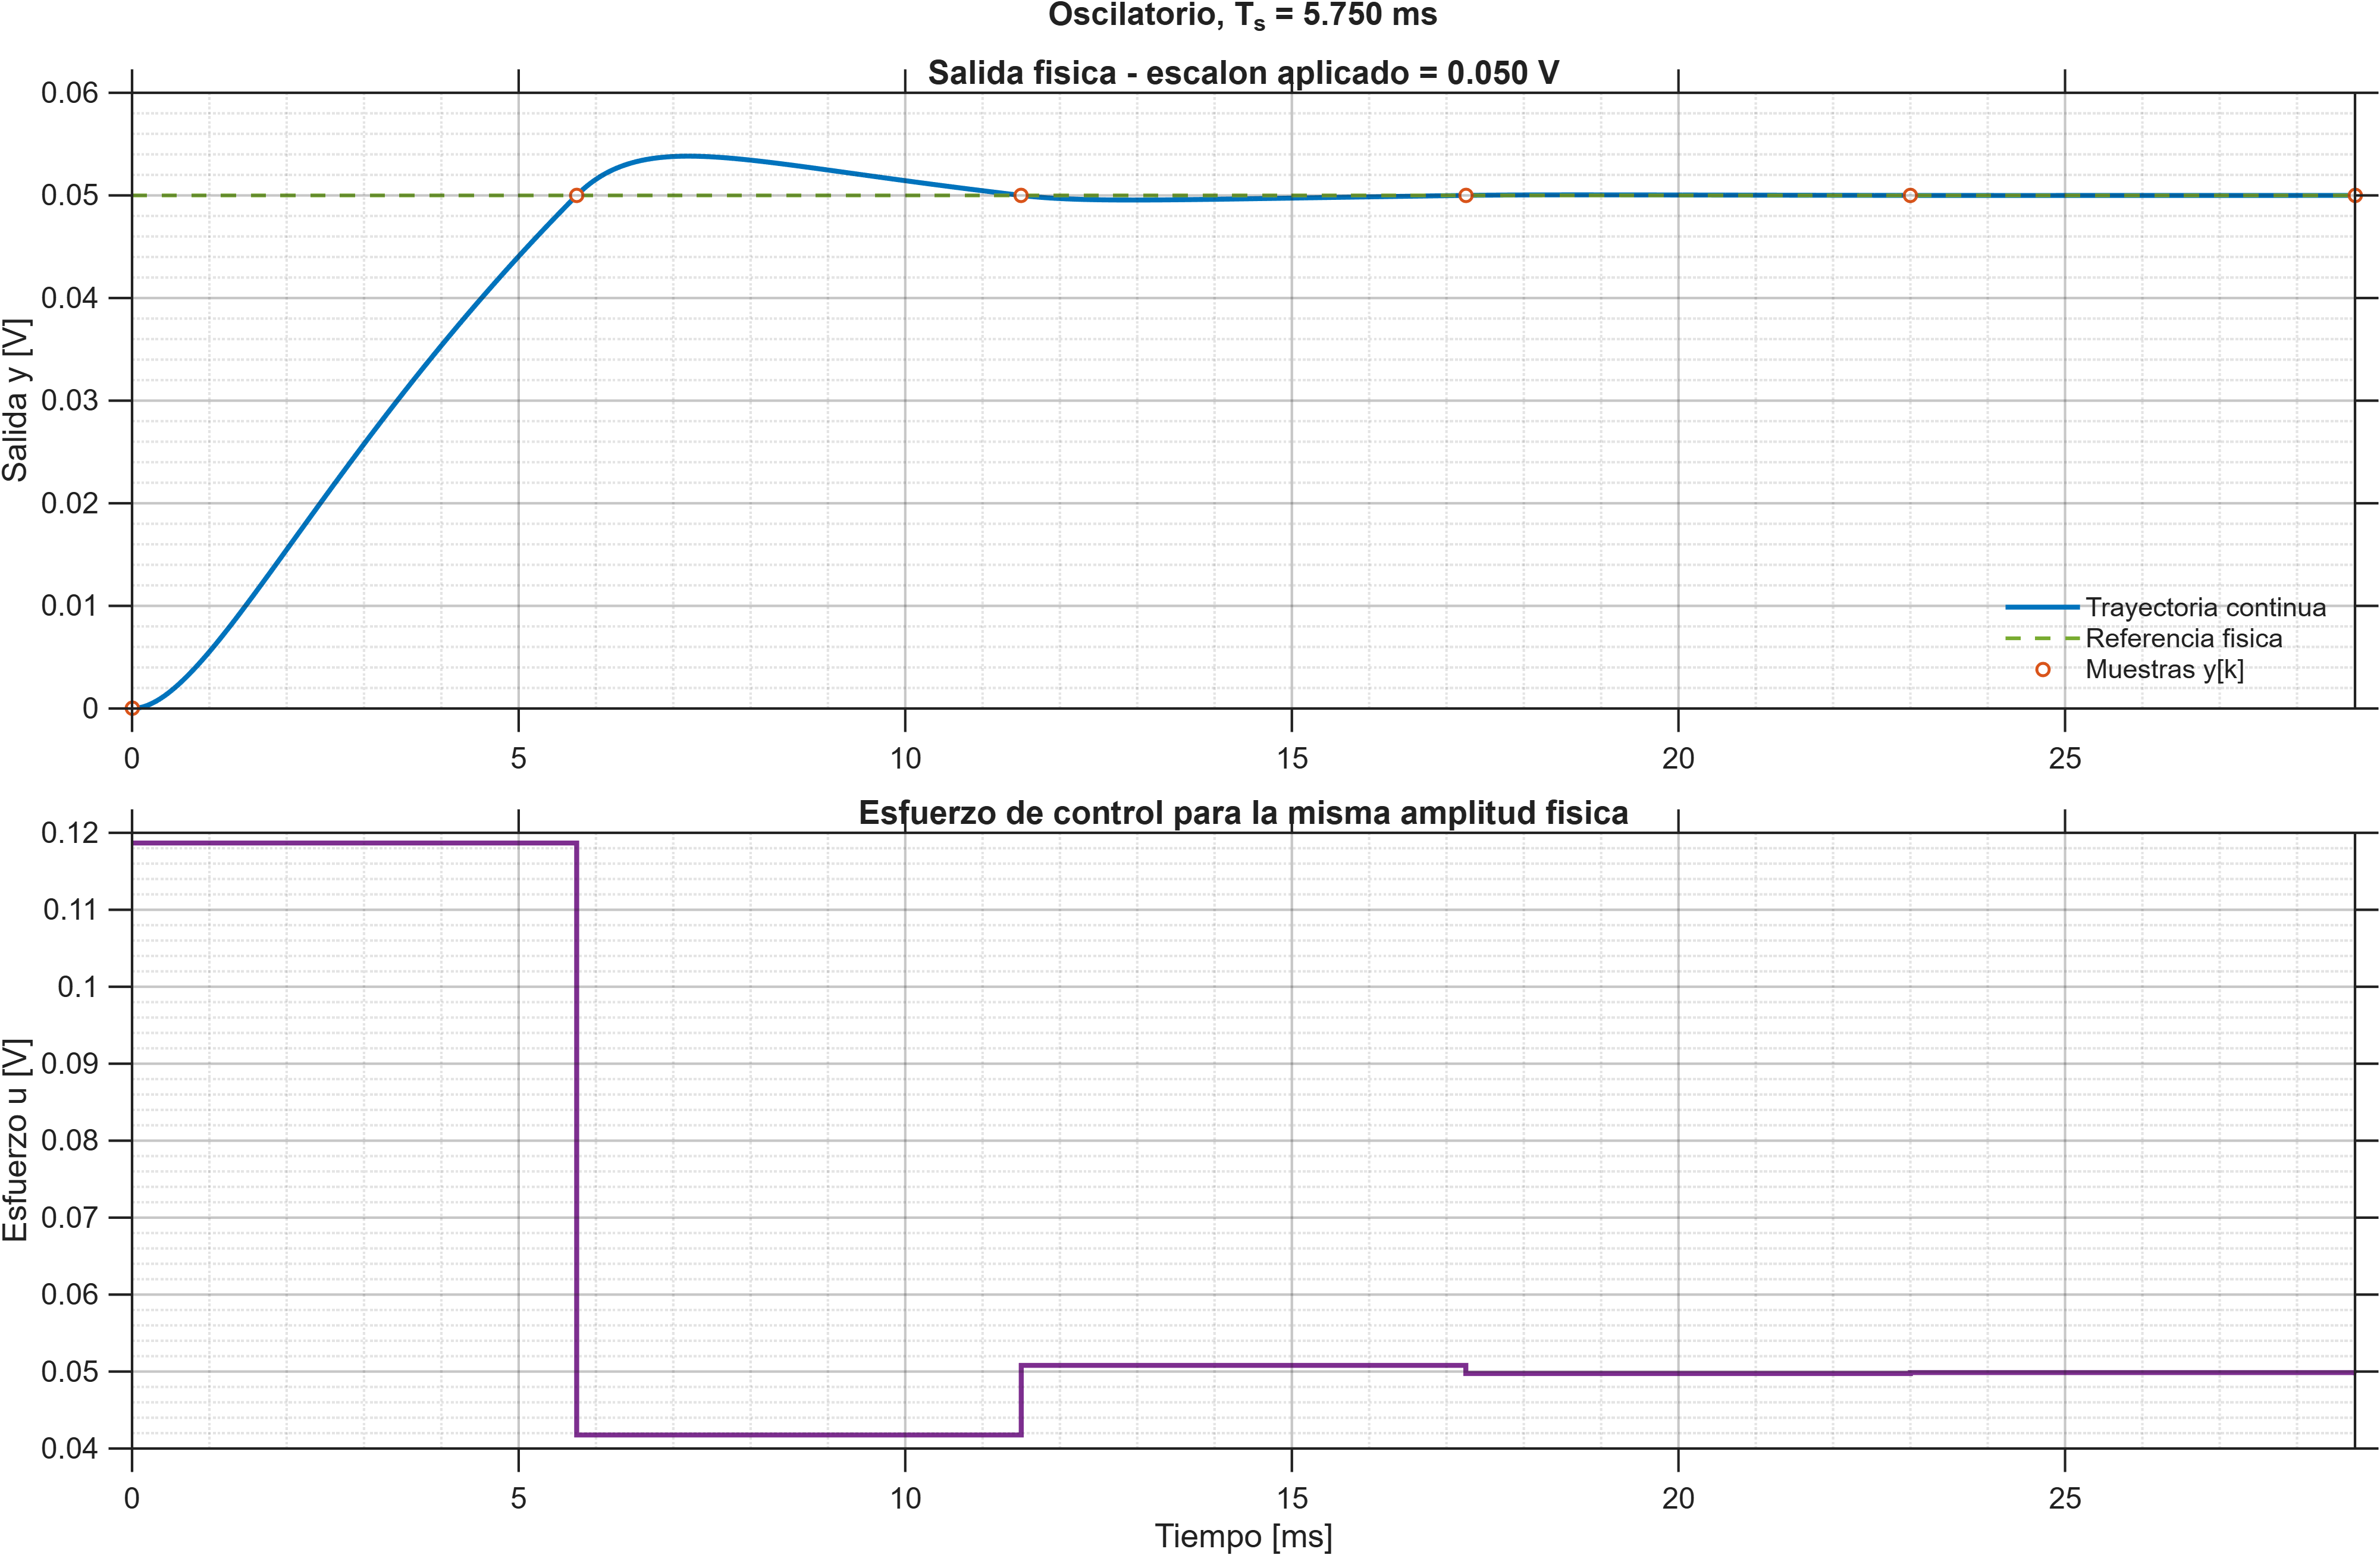
\includegraphics[width=0.76\textwidth]{respuesta_Ts1_oscilatorio.png}
\caption{Simulación continua y muestras para TS1, diseño oscilatorio.}
\vspace{6pt}
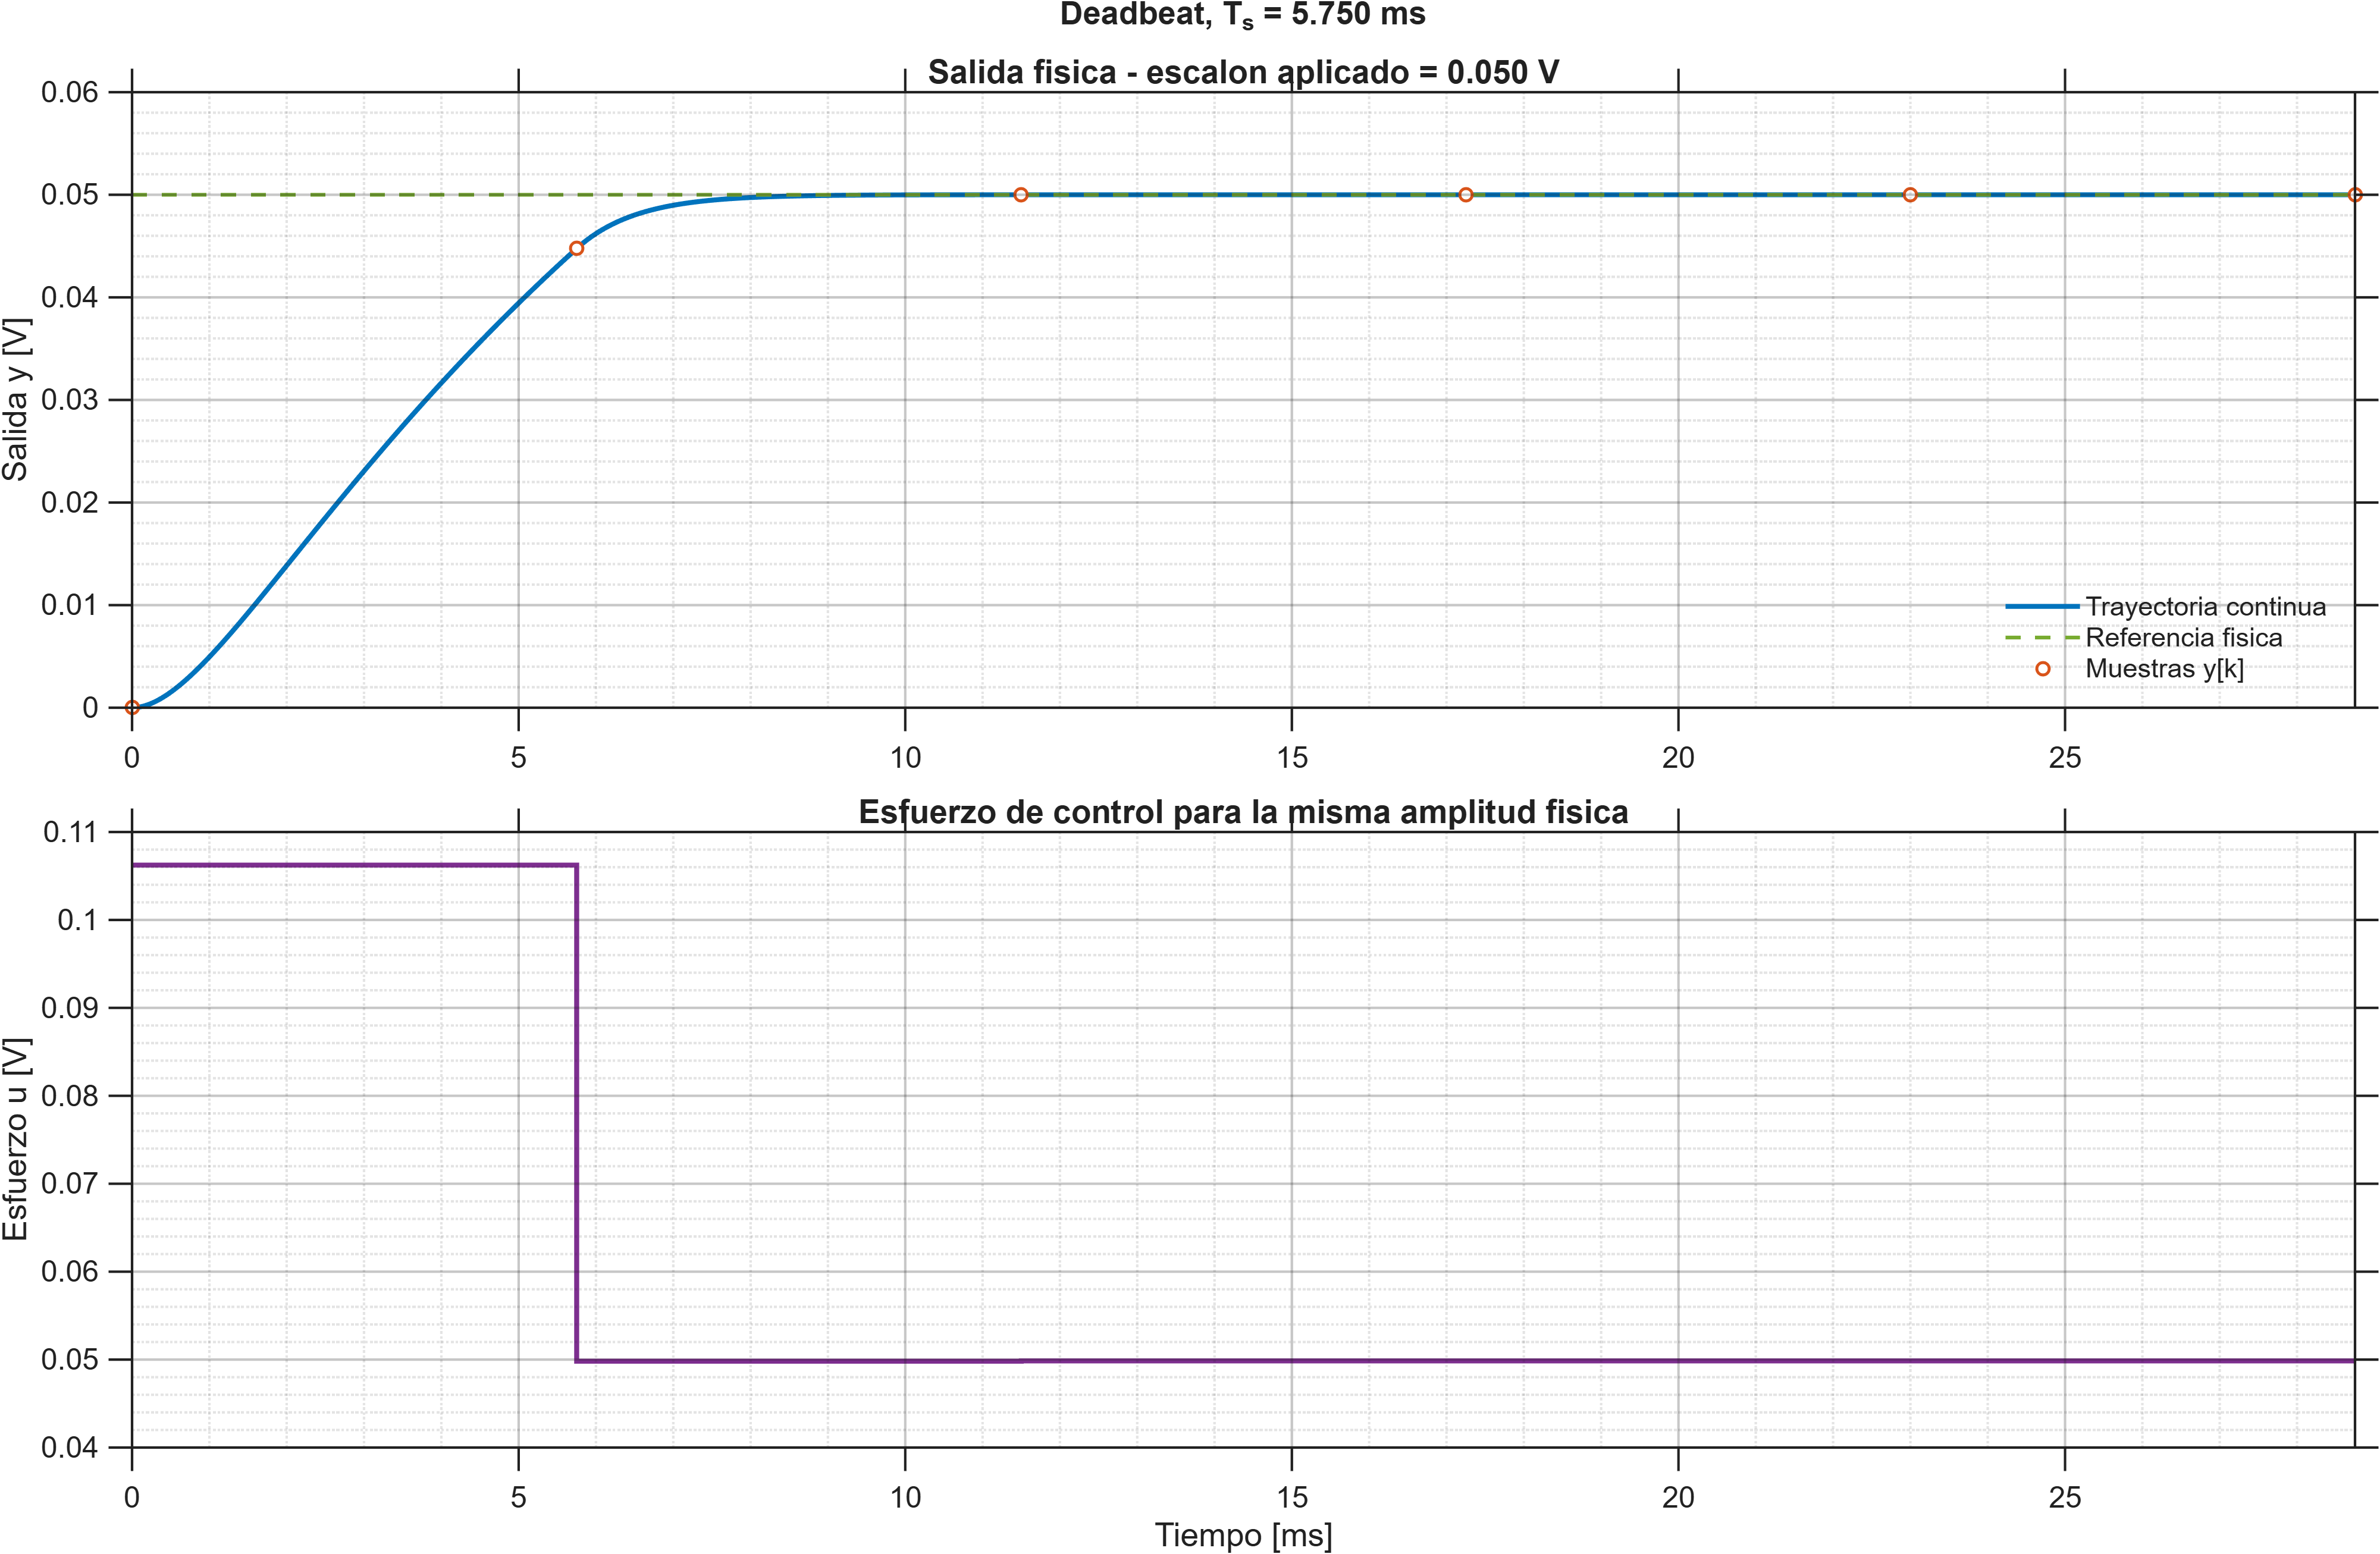
\includegraphics[width=0.76\textwidth]{respuesta_Ts1_deadbeat.png}
\caption{Simulación para TS1 con restricción deadbeat.}
\end{figure*}
\begin{figure*}[!p]
\centering
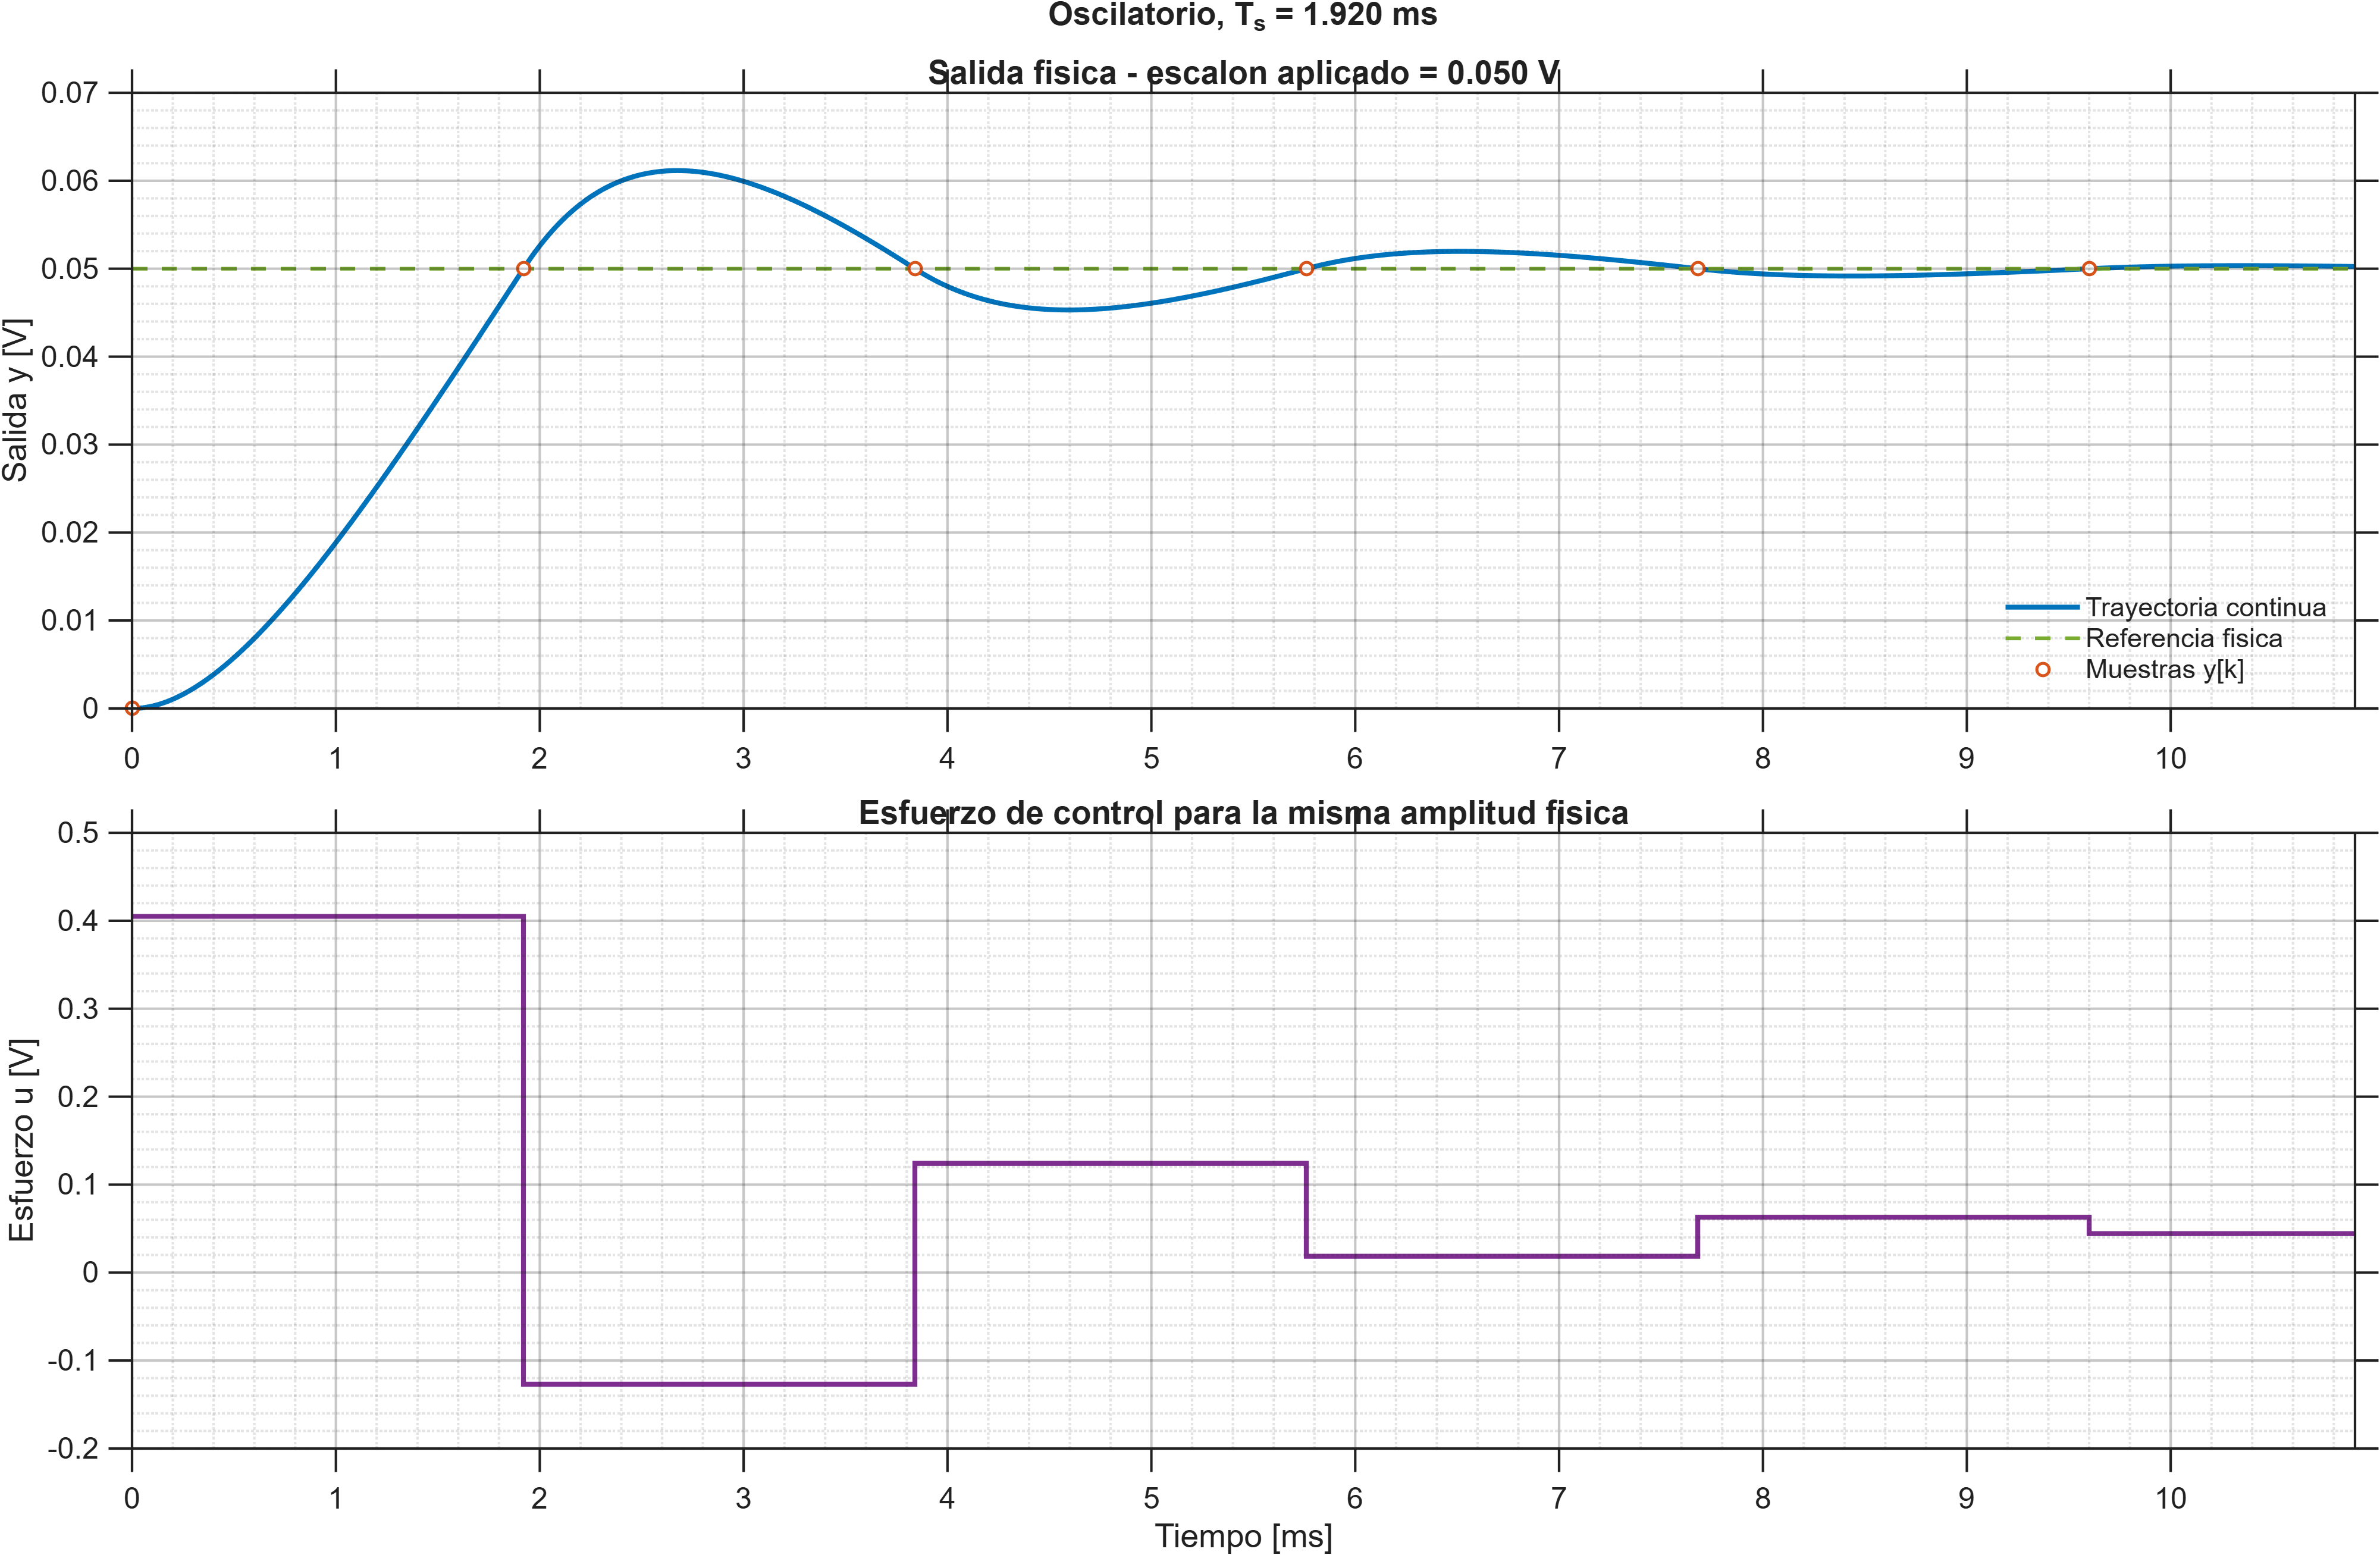
\includegraphics[width=0.76\textwidth]{respuesta_Ts2_oscilatorio.png}
\caption{Simulación para TS2; las muestras ocultan la excursión intramuestra.}
\vspace{6pt}
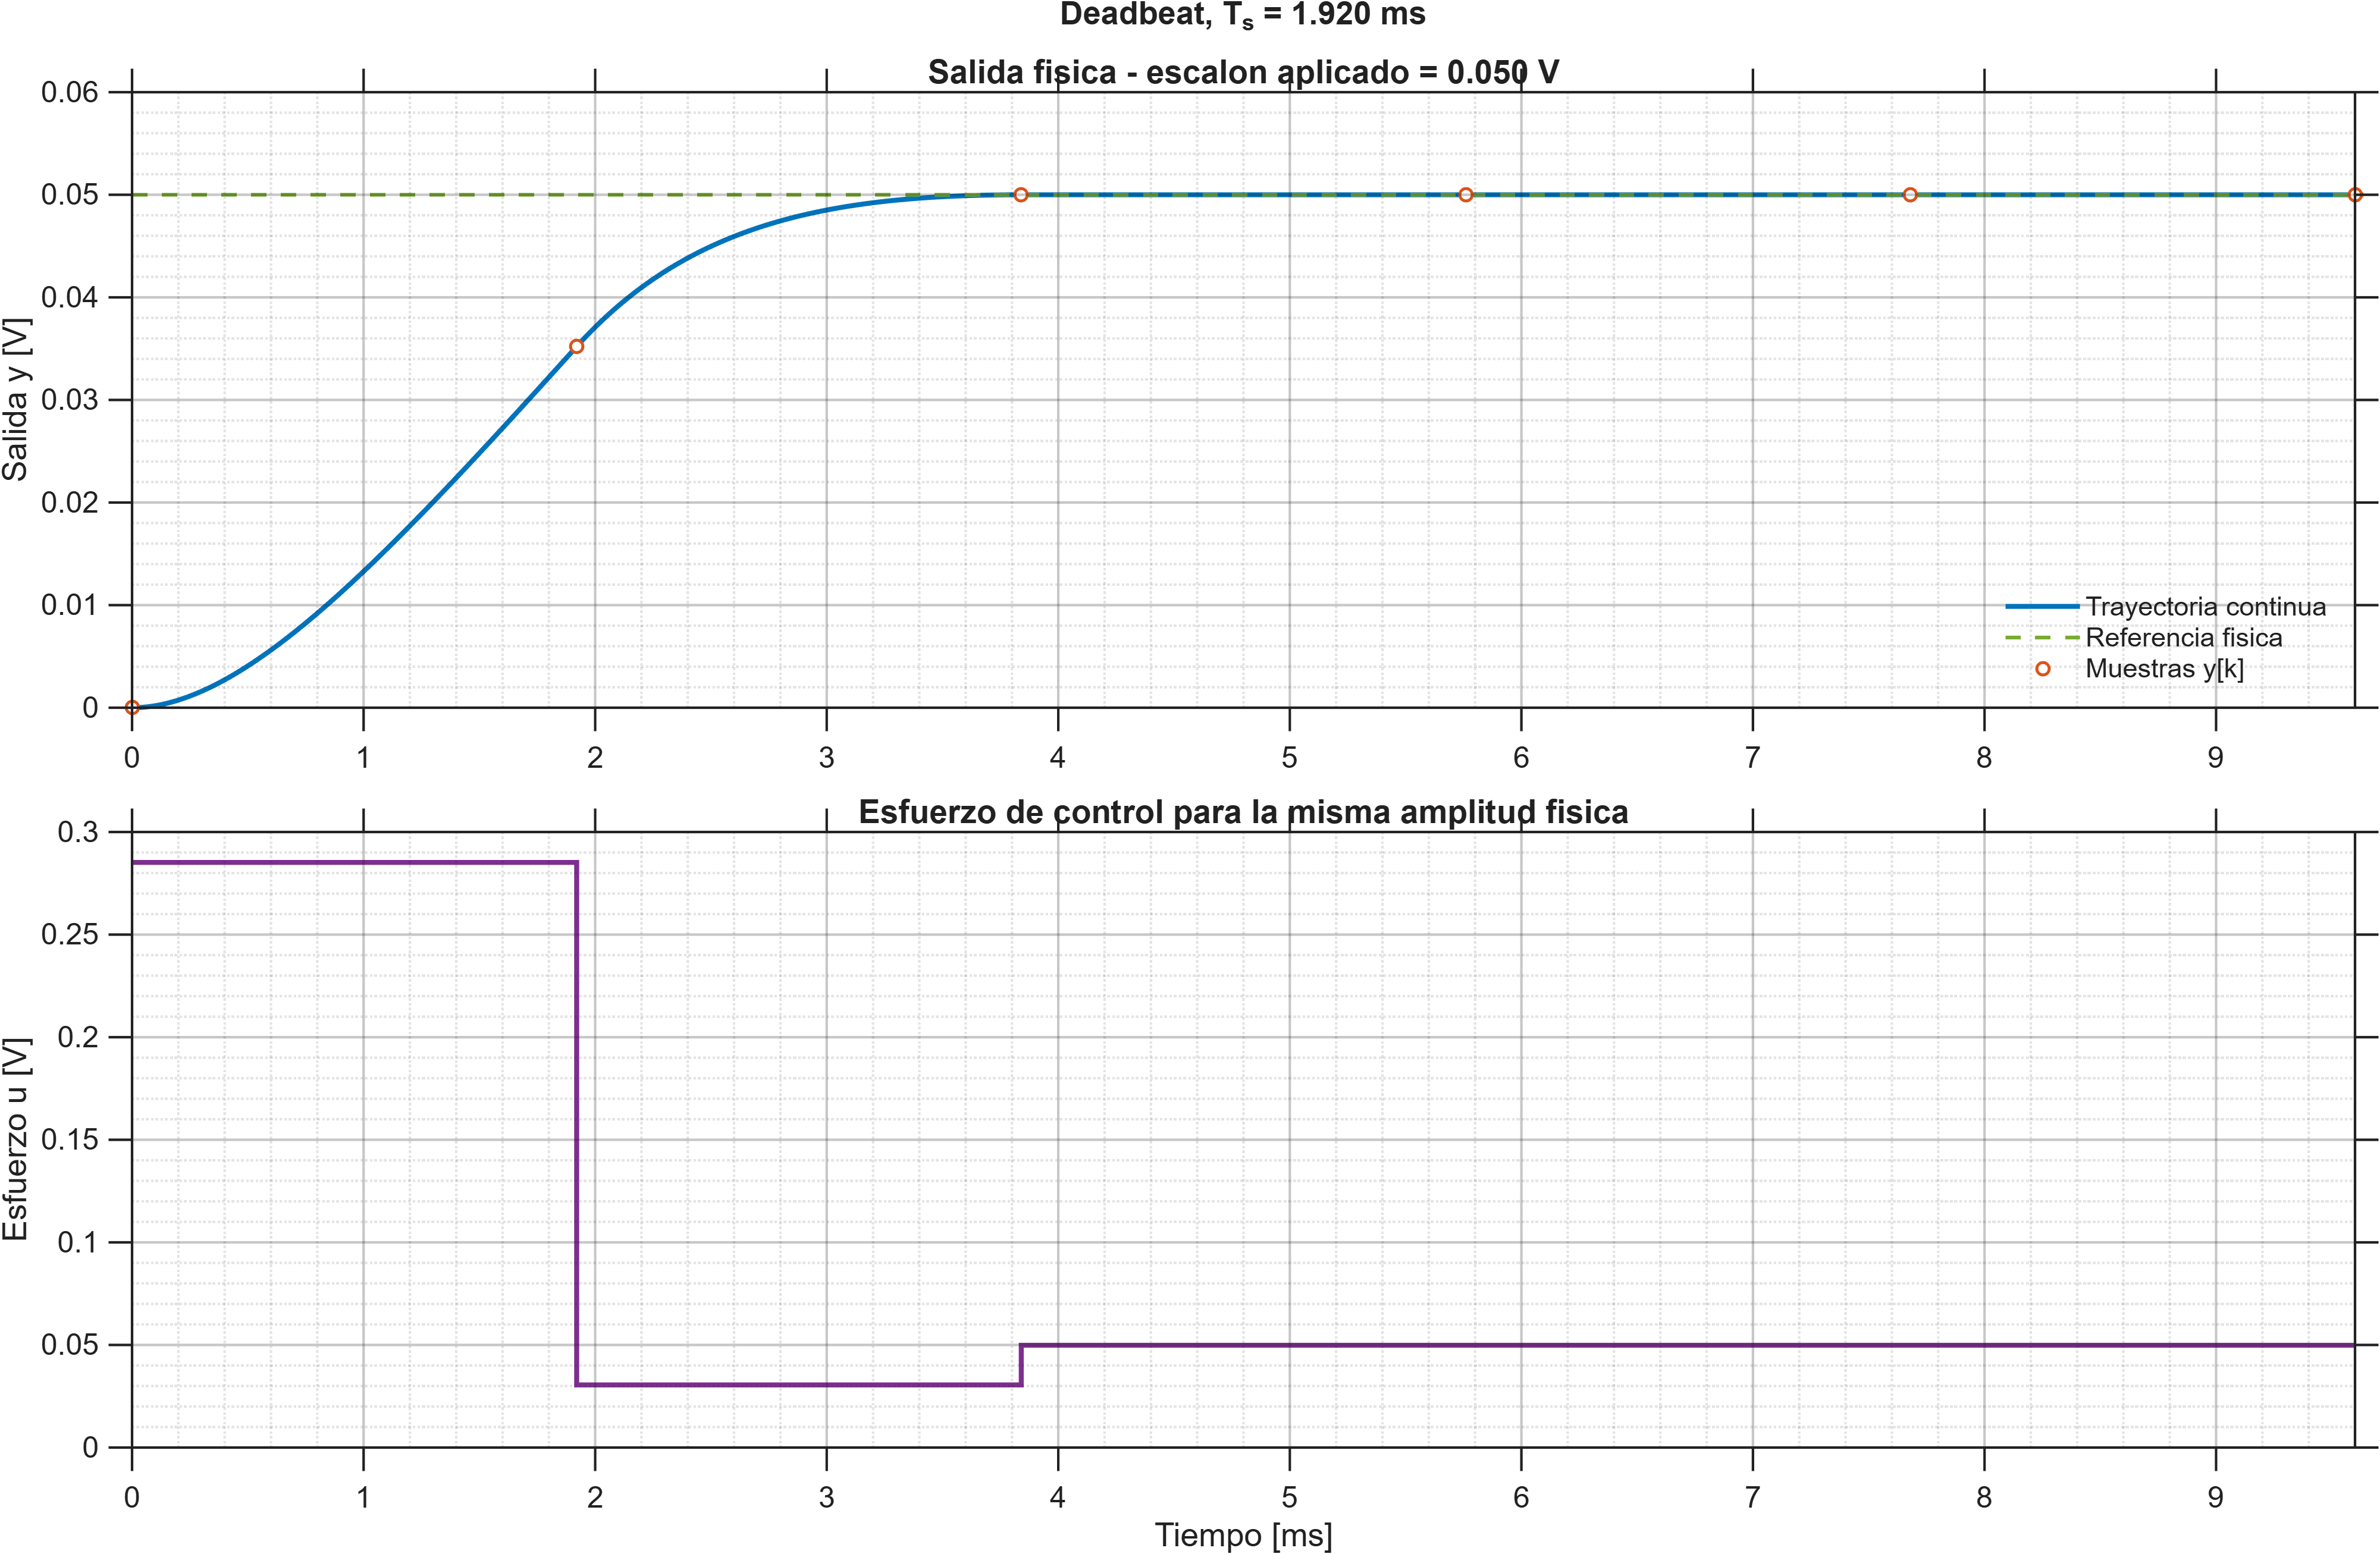
\includegraphics[width=0.76\textwidth]{respuesta_Ts2_deadbeat.png}
\caption{Simulación para TS2 con eliminación del rizado determinista.}
\end{figure*}
\begin{figure*}[!p]
\centering
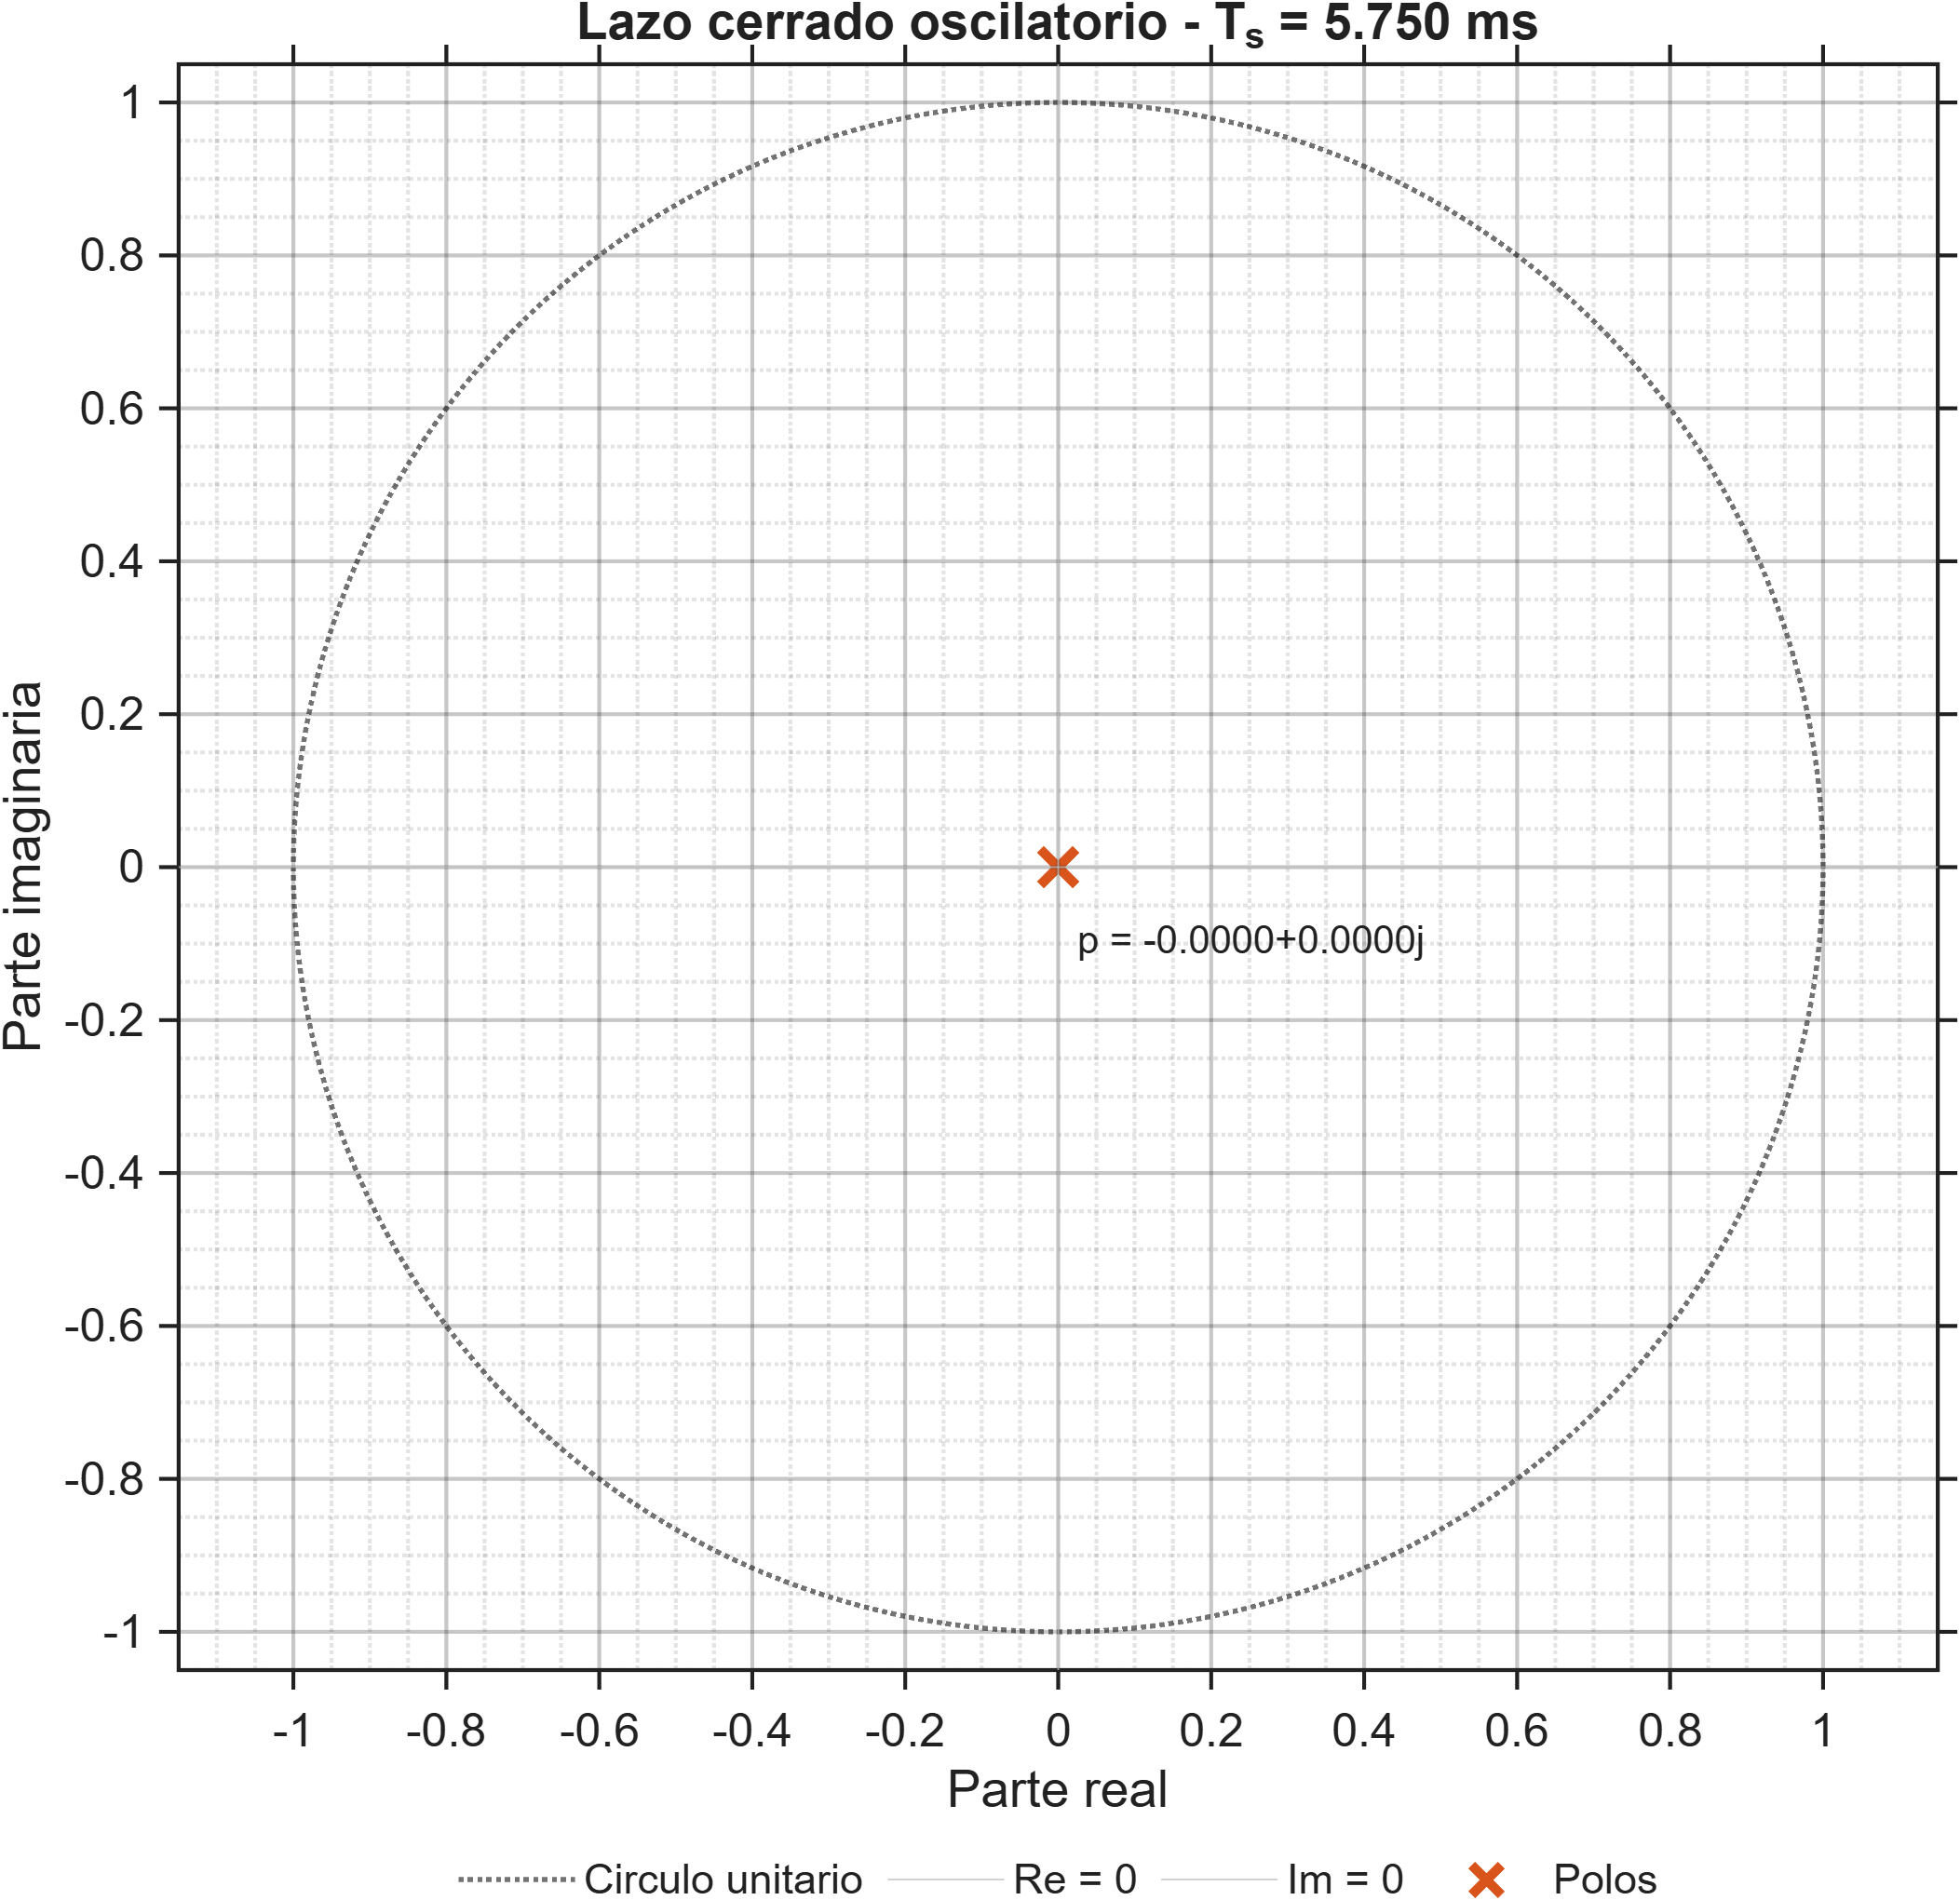
\includegraphics[width=0.48\textwidth]{pz_lazo_Ts1_oscilatorio.png}
\caption{Polos y ceros del lazo cerrado, TS1 oscilatorio.}
\vspace{5pt}
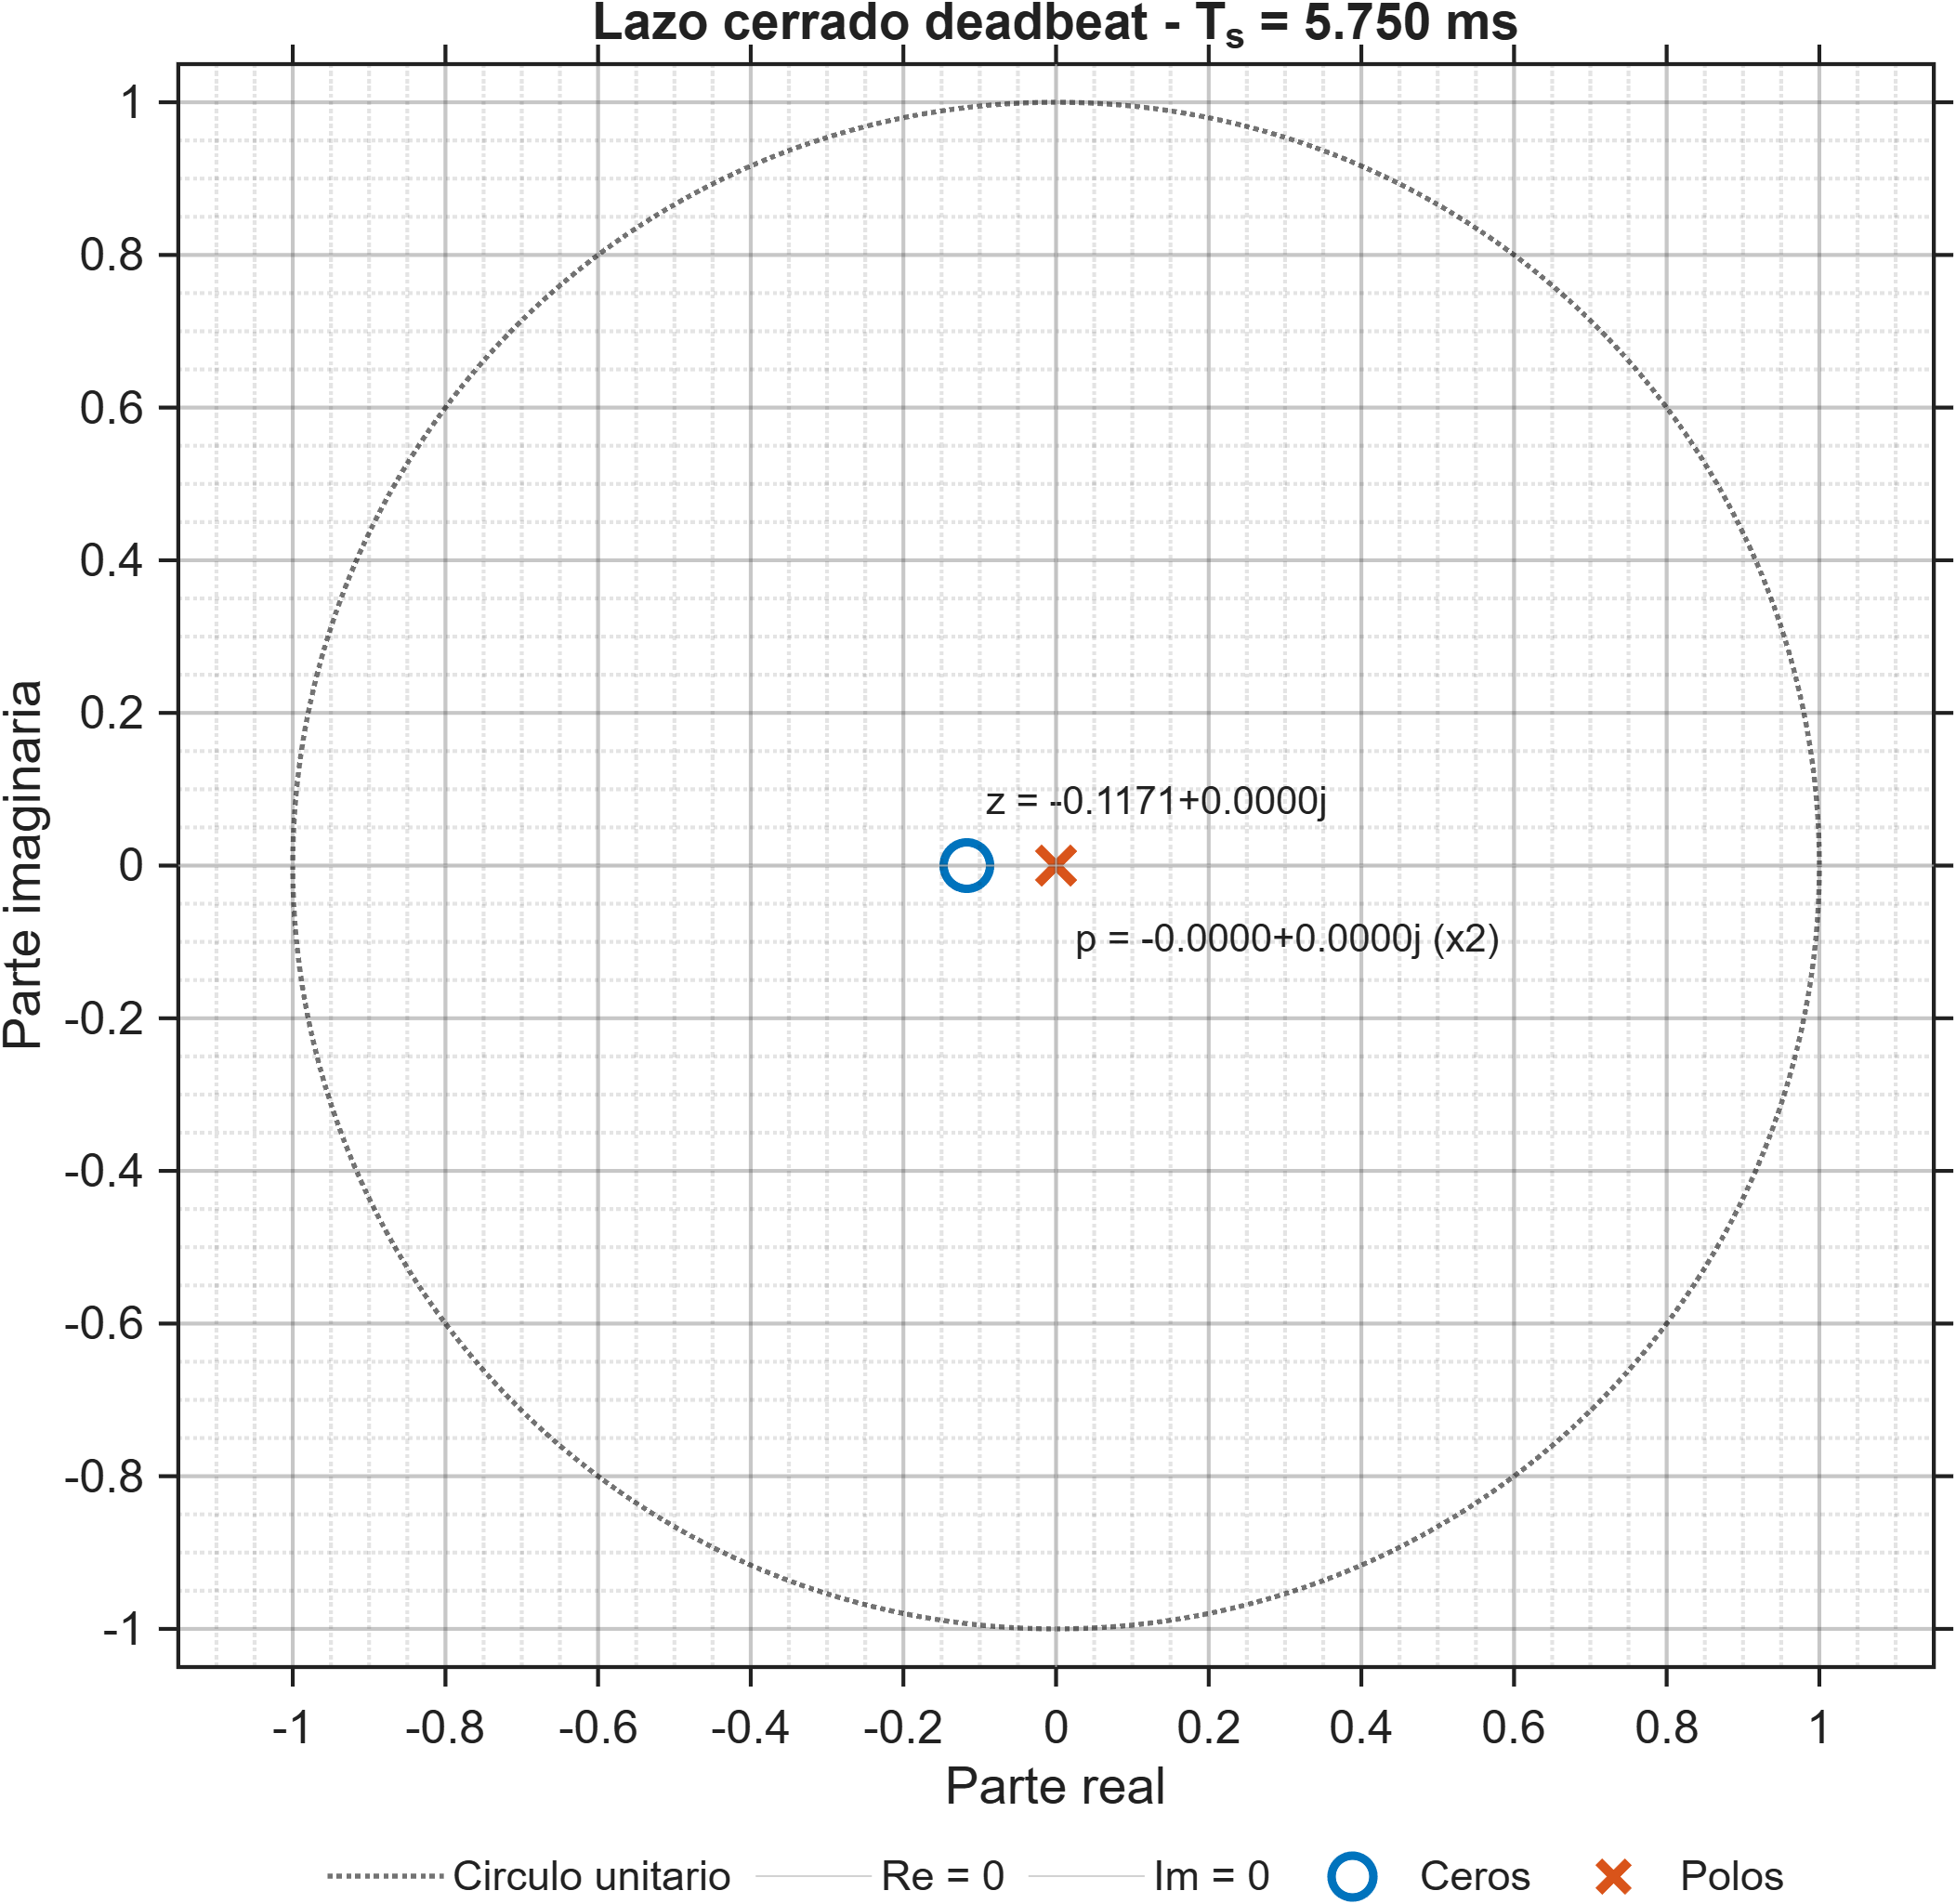
\includegraphics[width=0.48\textwidth]{pz_lazo_Ts1_deadbeat.png}
\caption{Polos y ceros del lazo cerrado, TS1 deadbeat.}
\end{figure*}
\begin{figure*}[!p]
\centering
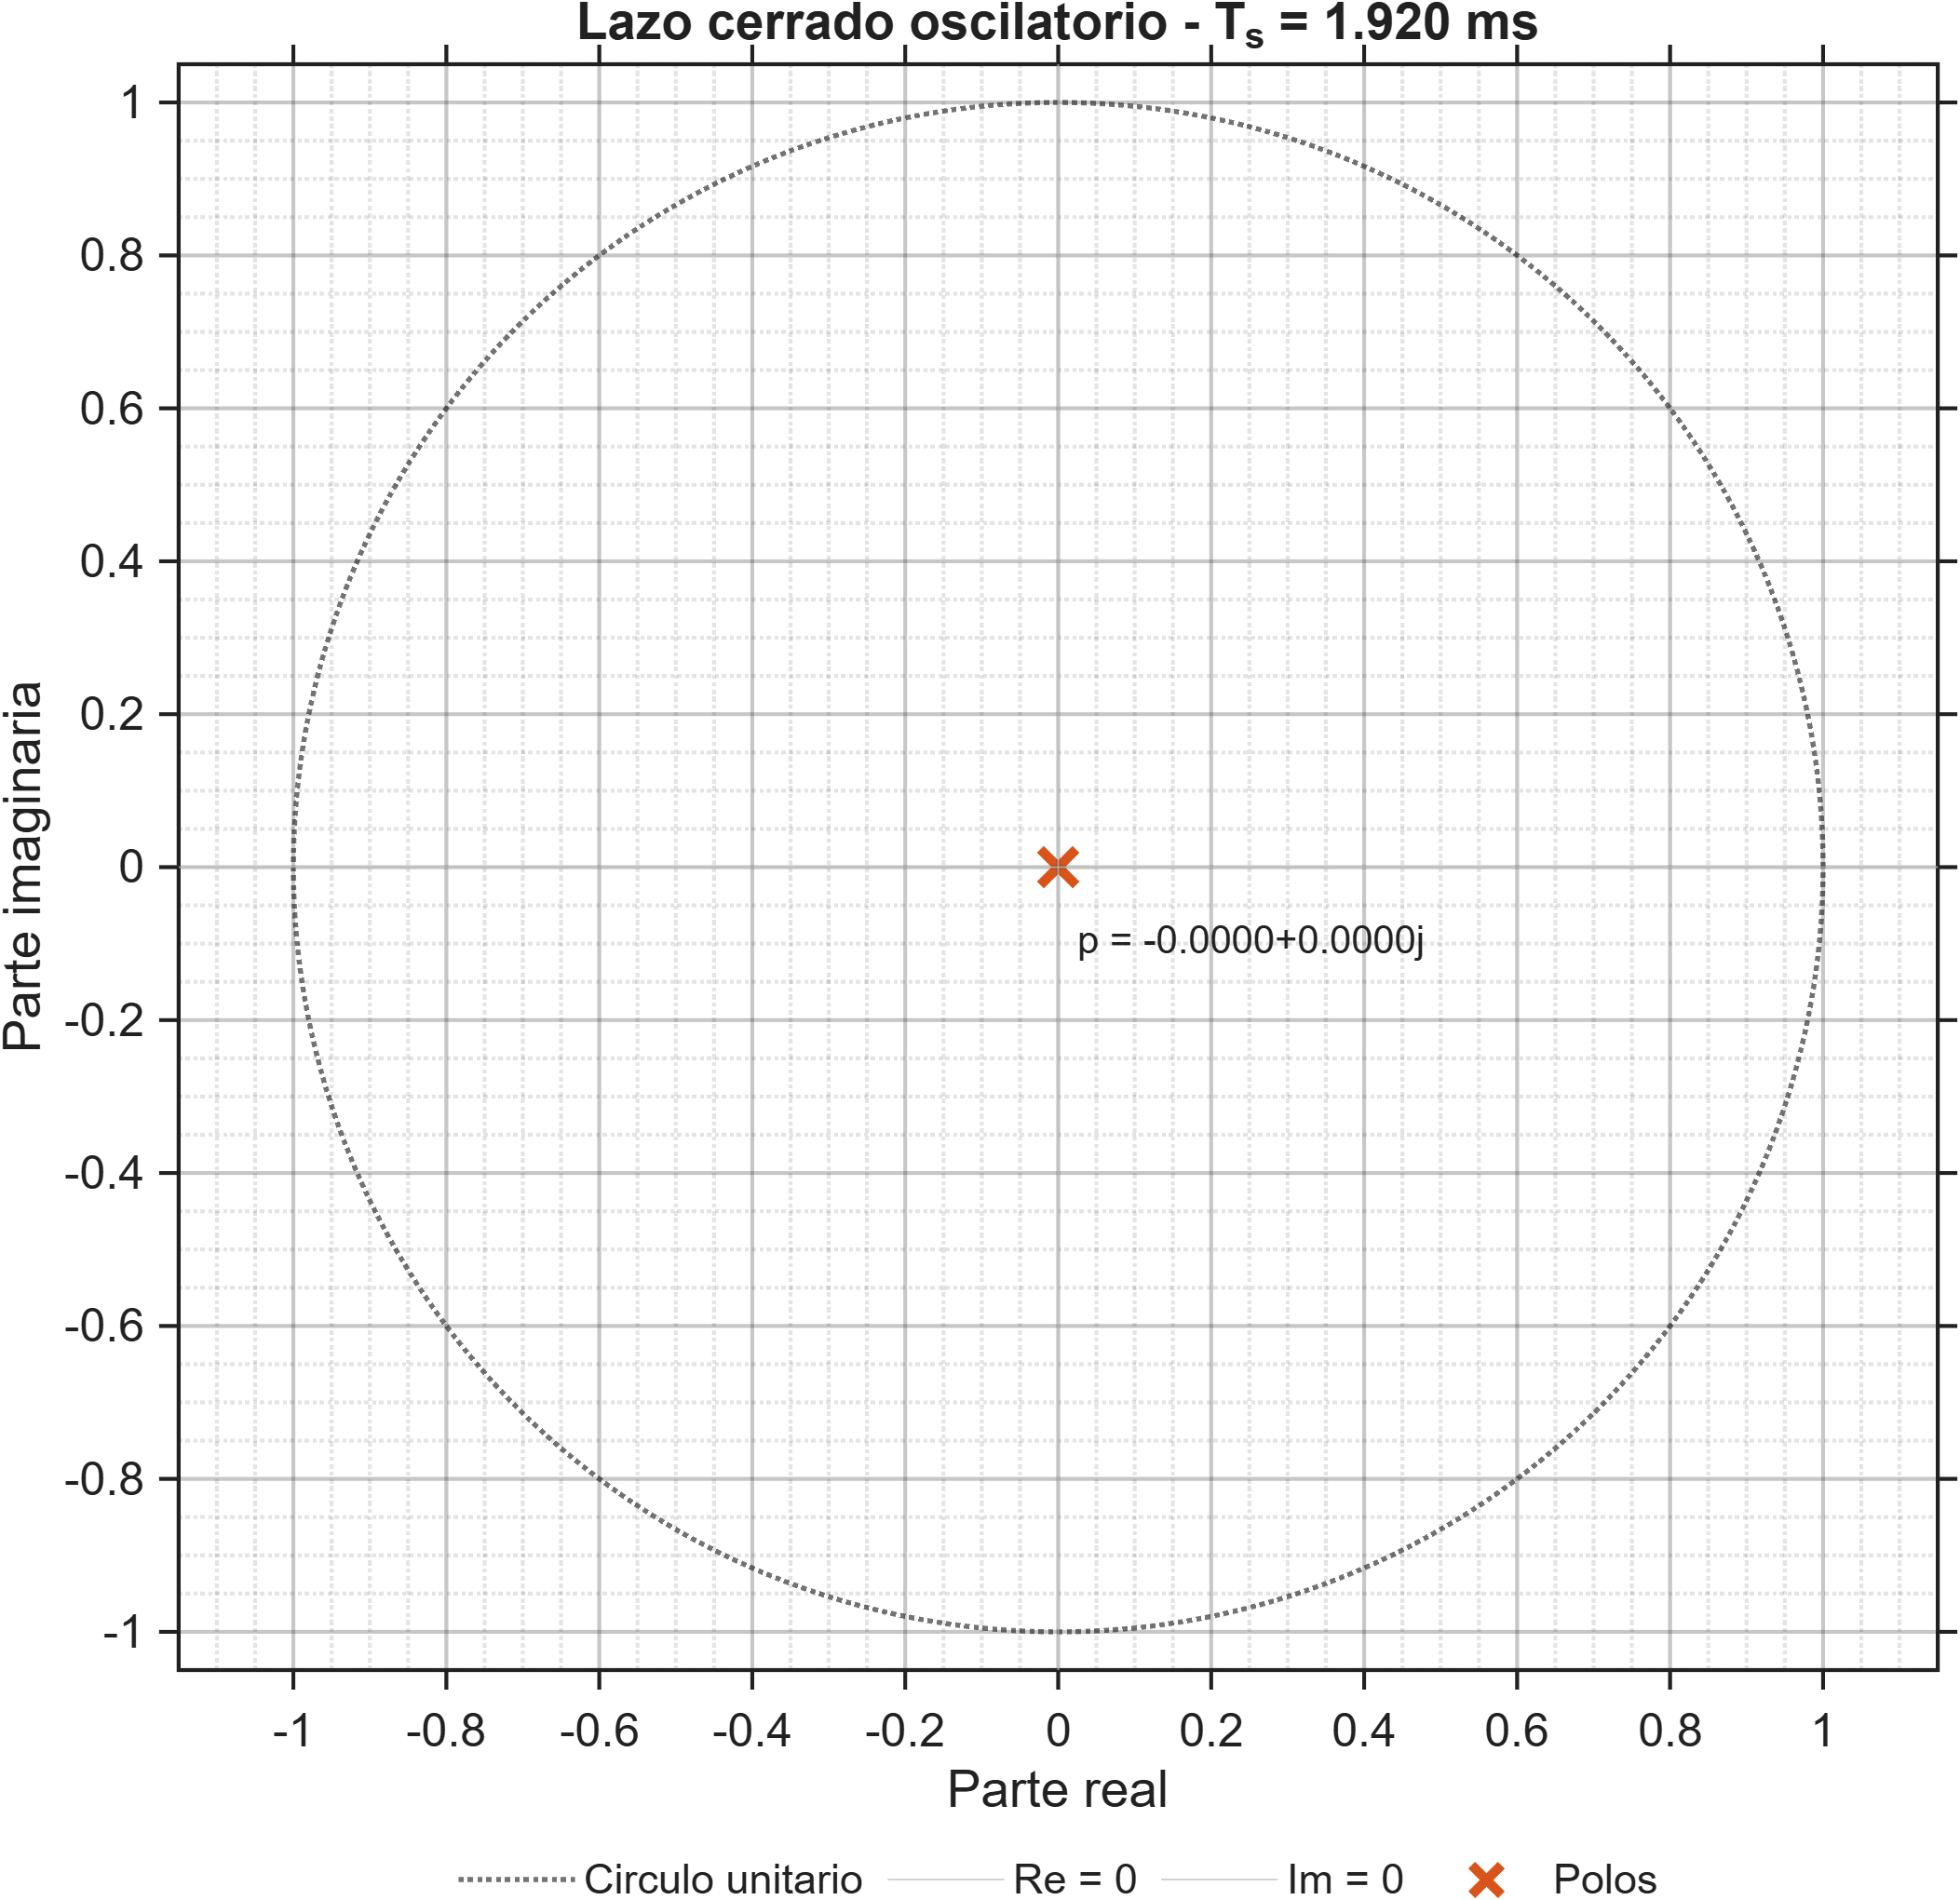
\includegraphics[width=0.48\textwidth]{pz_lazo_Ts2_oscilatorio.png}
\caption{Polos y ceros del lazo cerrado, TS2 oscilatorio.}
\vspace{5pt}
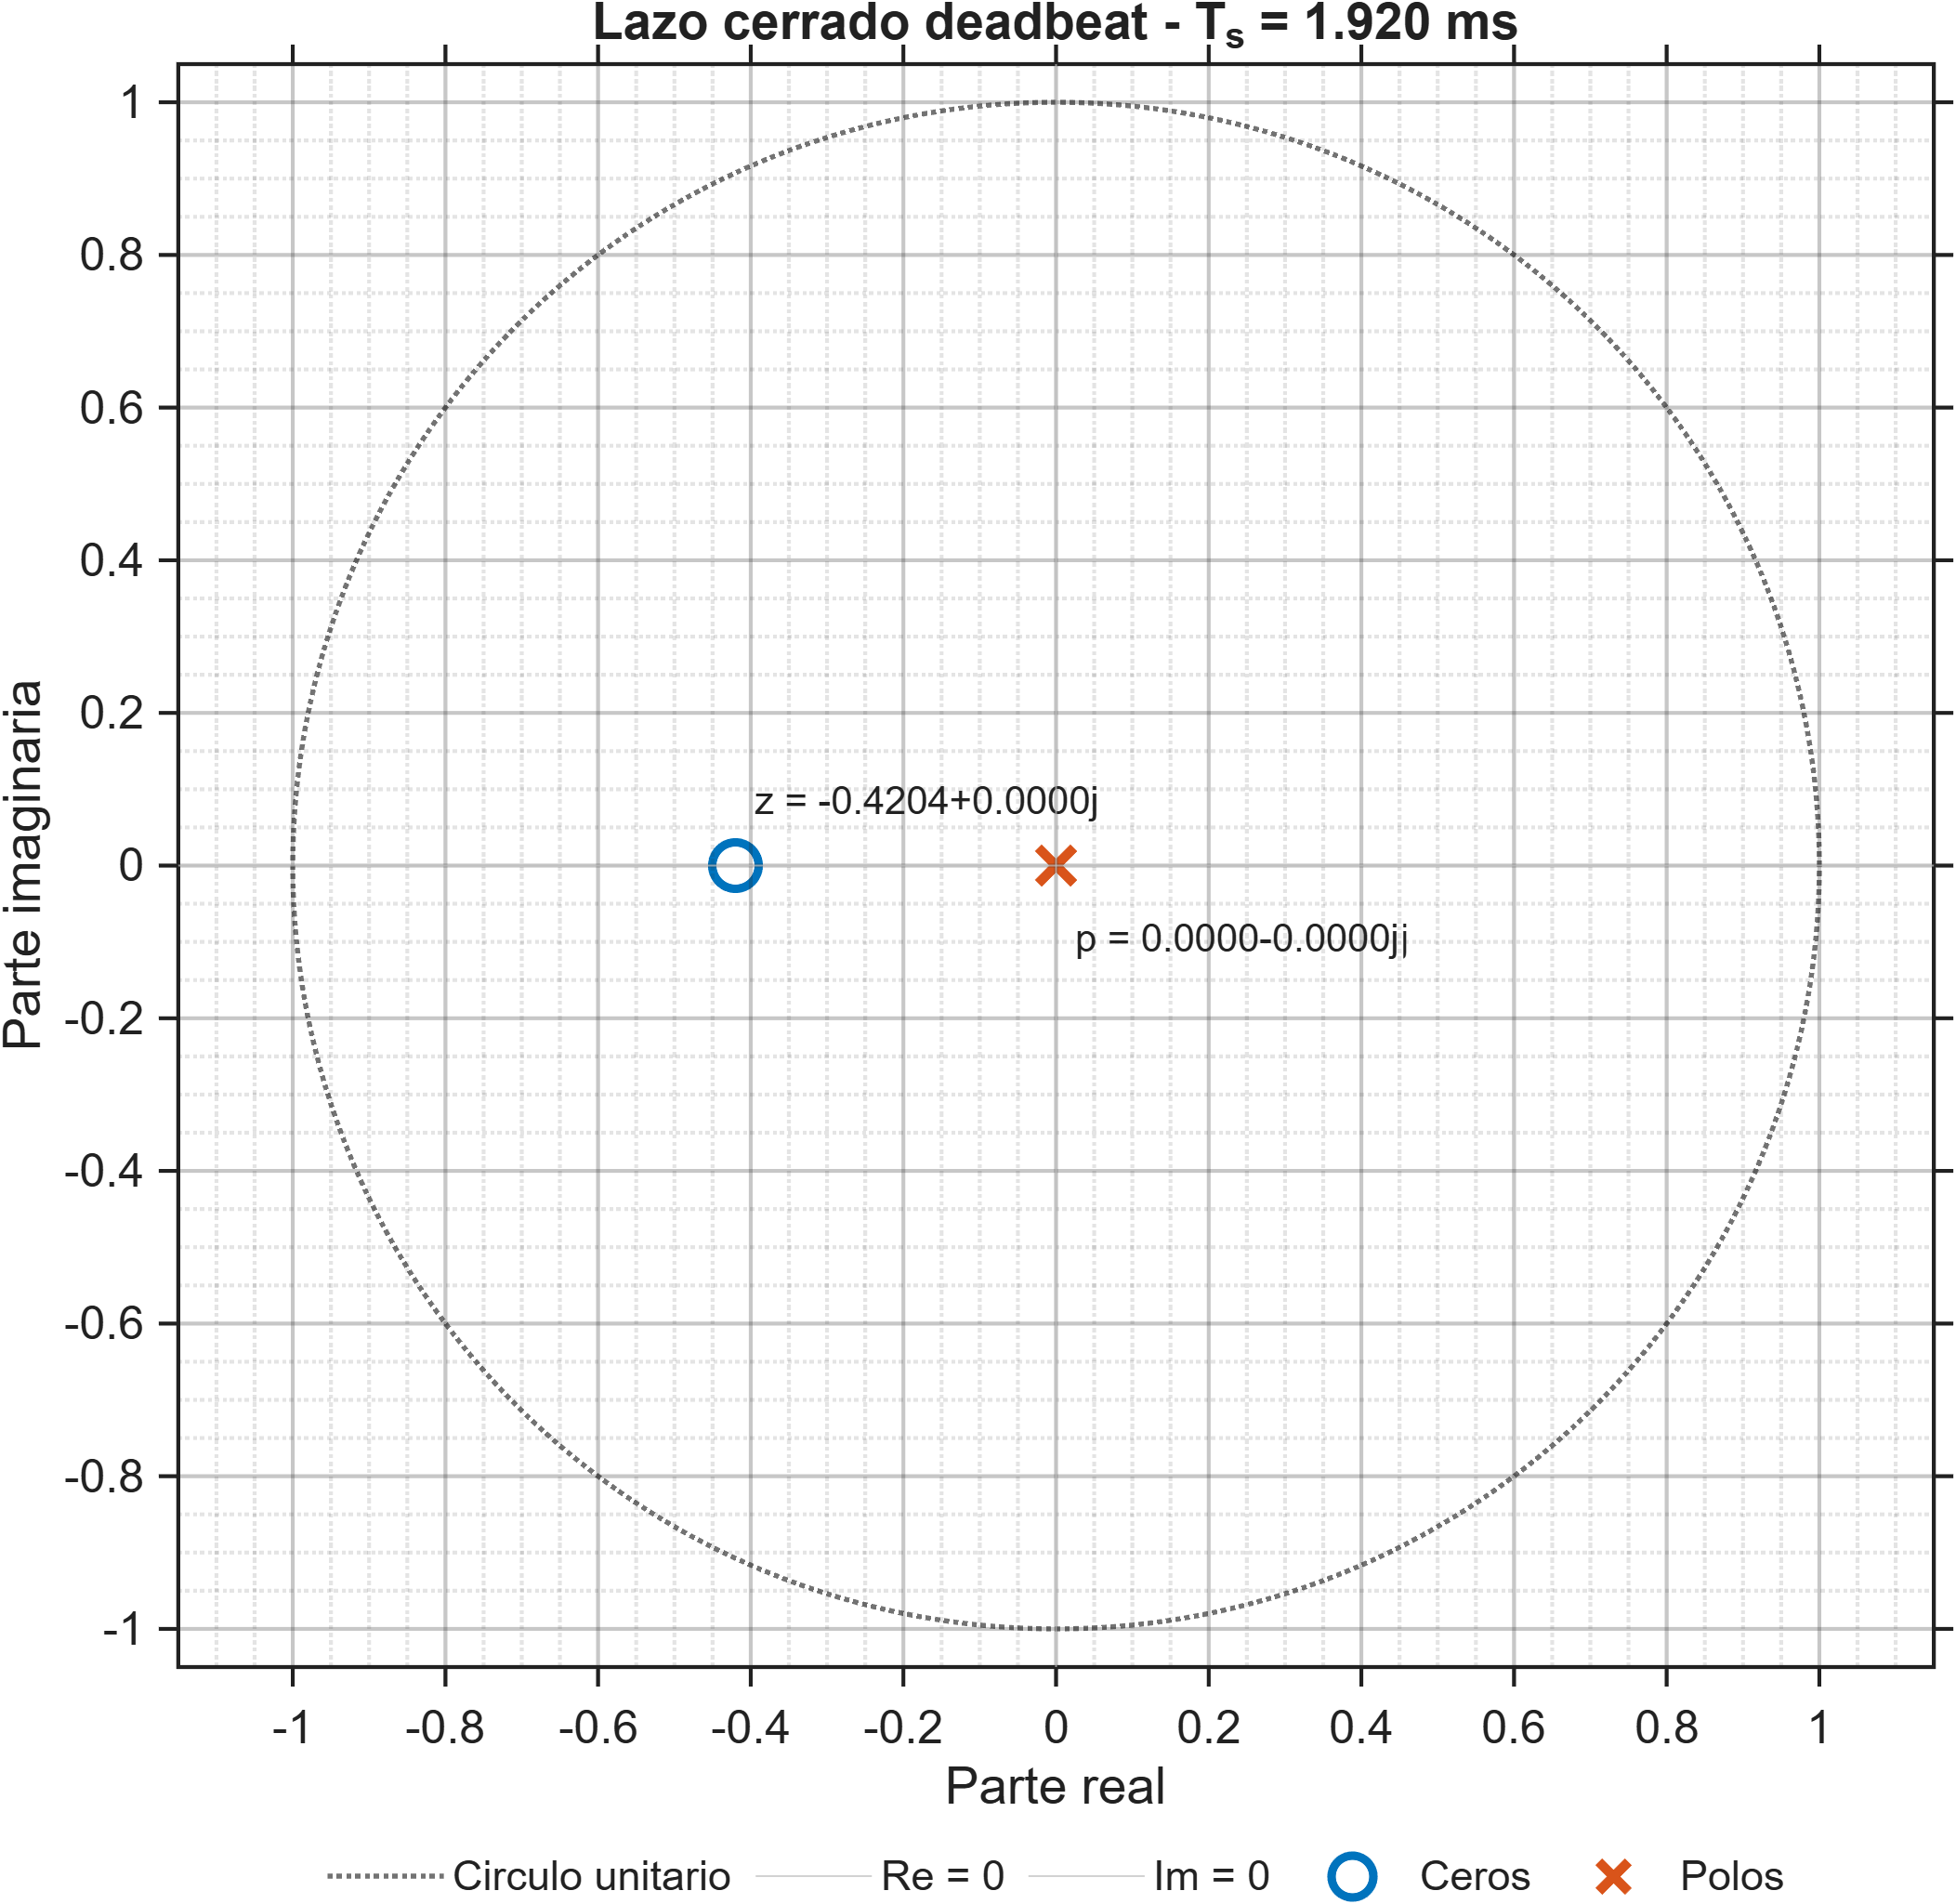
\includegraphics[width=0.48\textwidth]{pz_lazo_Ts2_deadbeat.png}
\caption{Polos y ceros del lazo cerrado, TS2 deadbeat.}
\end{figure*}
\clearpage
\nobalance

\section{Resultados}
\begin{table}[!h]
\centering
\caption{Comparación entre valores calculados, simulados y medidos para un escalón de 50 mV}
\label{tab:comparacion}
\resizebox{\columnwidth}{!}{%
\begin{tabular}{lrrrr}
\toprule
Magnitud & TS1-O & TS1-D & TS2-O & TS2-D\\
\midrule
\(z_0\) calculado & -0,1171 & -0,1171 & -0,4204 & -0,4204\\
\(t_s\) simulado (ms) & 10,435 & 7,018 & 7,269 & 3,128\\
\(M_p\) simulado (\%) & 7,653 & 0 & 22,312 & 0\\
\(u_{\max}\) simulado (mV) & 118,7 & 106,2 & 405,1 & 285,2\\
\(u_{\max}\) medido J5 (mV) & 134 & 120 & 456 & 312\\
\(y_{\max}\) medido J7 (mV) & 53,6 & 51,2 & 76,0 & 69,6\\
\bottomrule
\end{tabular}
}
\end{table}

La Tabla \ref{tab:comparacion} concentra la relación principal del laboratorio. El cero calculado se acerca a \(z=-1\) al reducir \(\Ts\); simultáneamente, el diseño de una muestra exige más mando y desarrolla mayor sobrepaso intramuestra. Los máximos experimentales son superiores a los simulados entre 10 y 13\,\%, diferencia compatible con cuantización, ruido de medida, tolerancias del montaje y error de modelo, sin alterar la tendencia entre controladores.

La auditoría confirmó las cuatro identidades y sus coeficientes. En TS1, el máximo positivo continuo de J5 disminuyó de 134 a 120 mV al pasar del controlador oscilatorio al deadbeat, una reducción de 10,4\,\%. En las muestras del PSoC, el pico del mando aplicado pasó de 123 a 108 mV, equivalente a 12,2\,\%. En TS2, el máximo positivo continuo de J5 pasó de 456 a 312 mV, una reducción de 31,6\,\%. Los máximos continuos de J7 fueron 53,6; 51,2; 76,0 y 69,6 mV, respectivamente.

\subsection{Comparación continua entre simulación y experimento}
Las Figuras 9--12 emplean una ventana de 35 ms para TS1 y de 20 ms para TS2. Las señales experimentales se conservan en voltios físicos. La simulación se traslada únicamente al nivel inicial medido, sin corrección de ganancia. Las nuevas capturas TS1 se dispararon en el transitorio y contienen, de forma independiente, los controladores oscilatorio y deadbeat.

\begin{figure*}[!p]
\centering
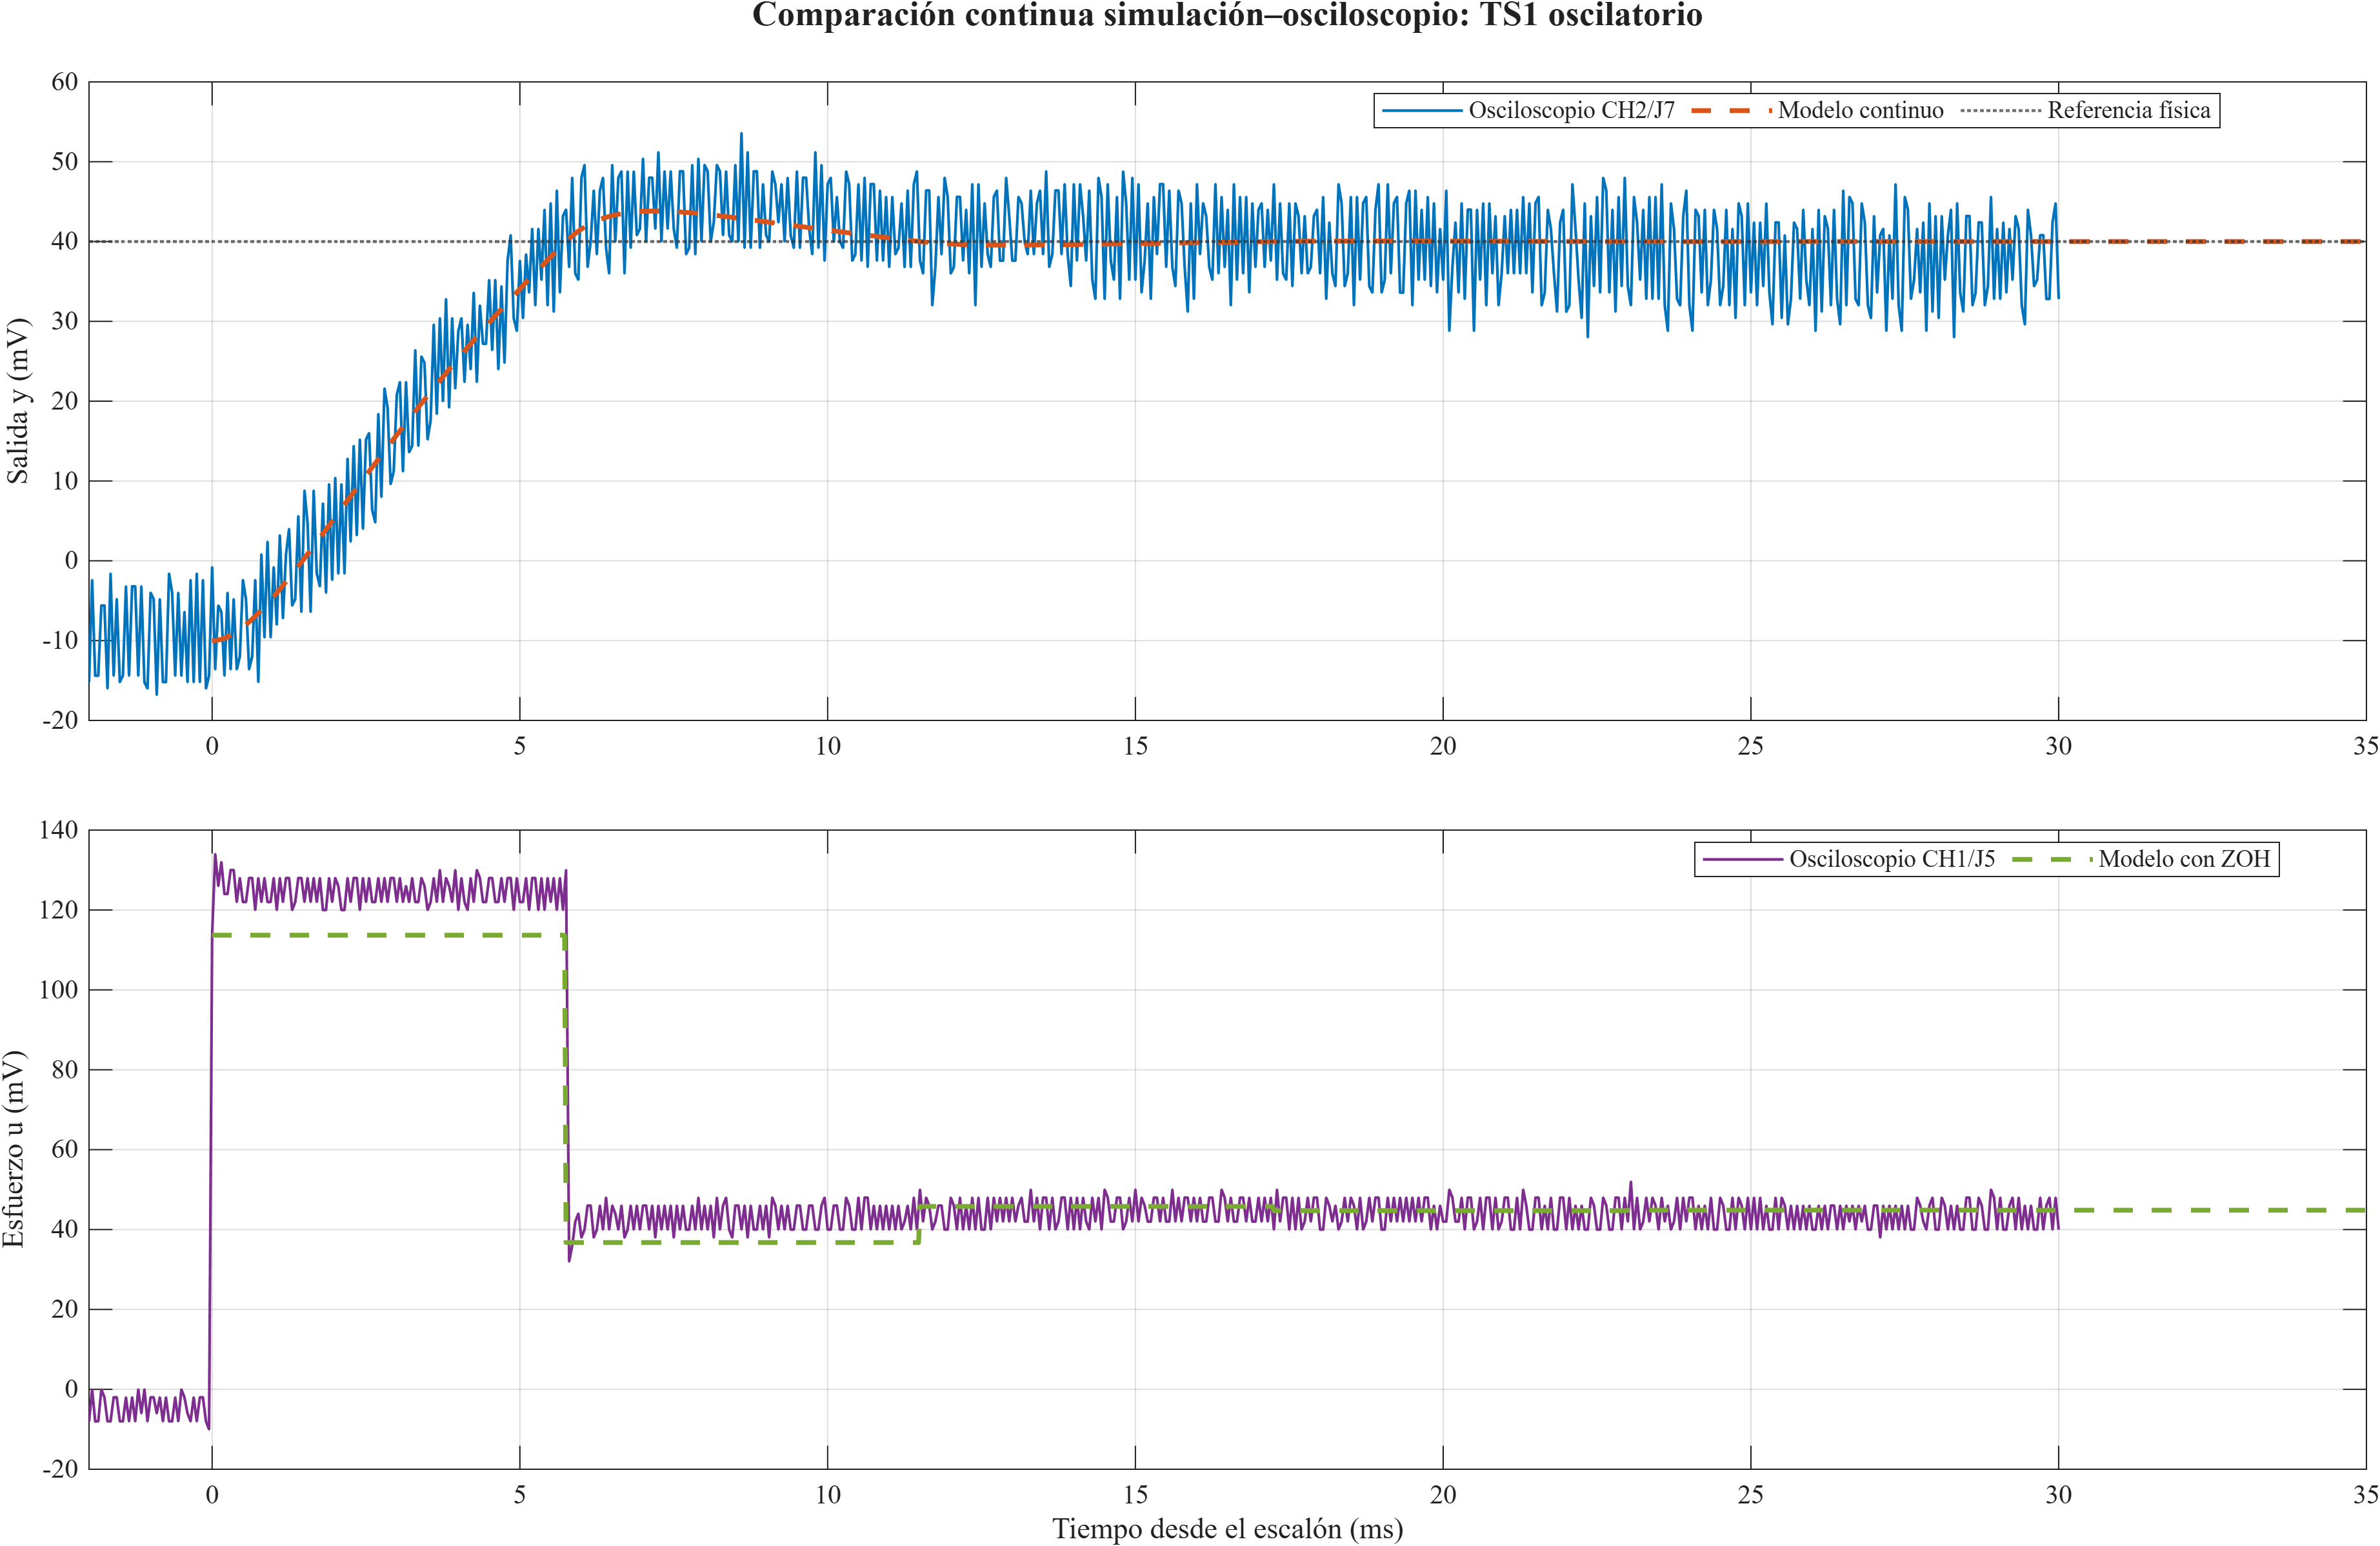
\includegraphics[width=0.78\textwidth]{comparacion_continua_ts1_oscilatorio.png}
\caption{Comparación continua modelo--osciloscopio para TS1 oscilatorio: salida en J7 y esfuerzo de control en J5.}
\vspace{6pt}
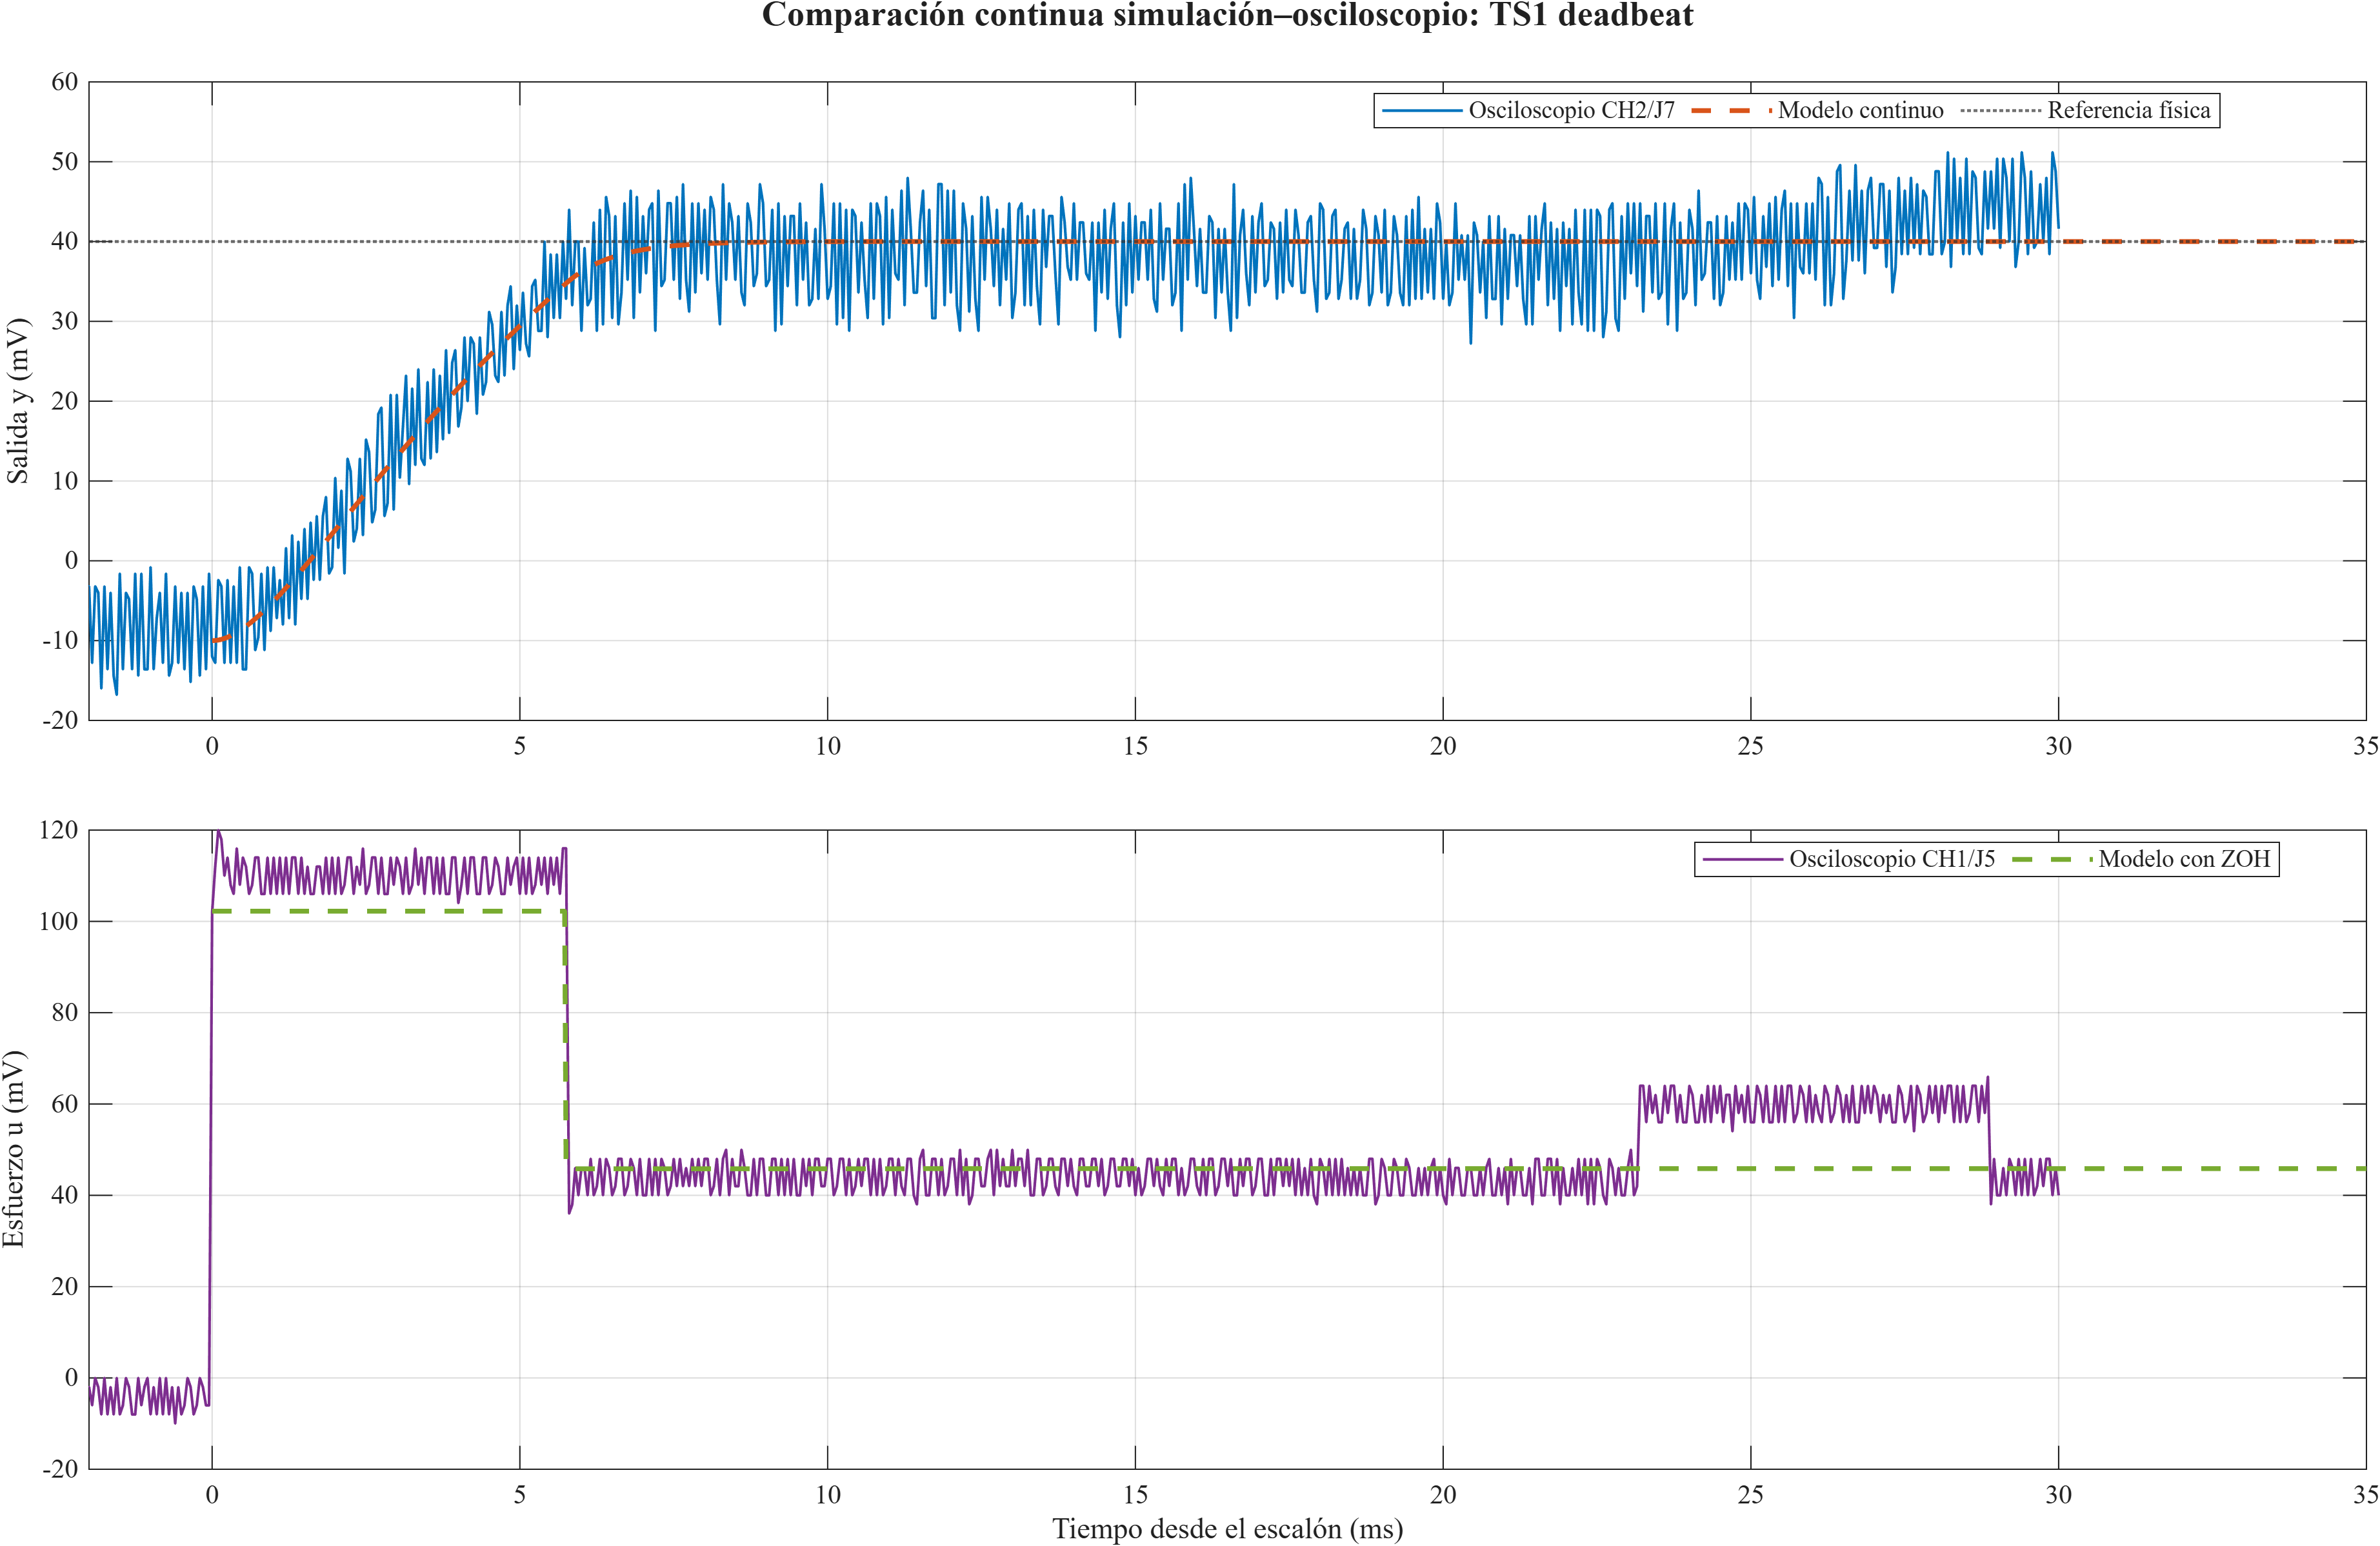
\includegraphics[width=0.78\textwidth]{comparacion_continua_ts1_deadbeat.png}
\caption{Comparación continua modelo--osciloscopio para TS1 deadbeat: salida en J7 y esfuerzo de control en J5.}
\end{figure*}

\begin{figure*}[!p]
\centering
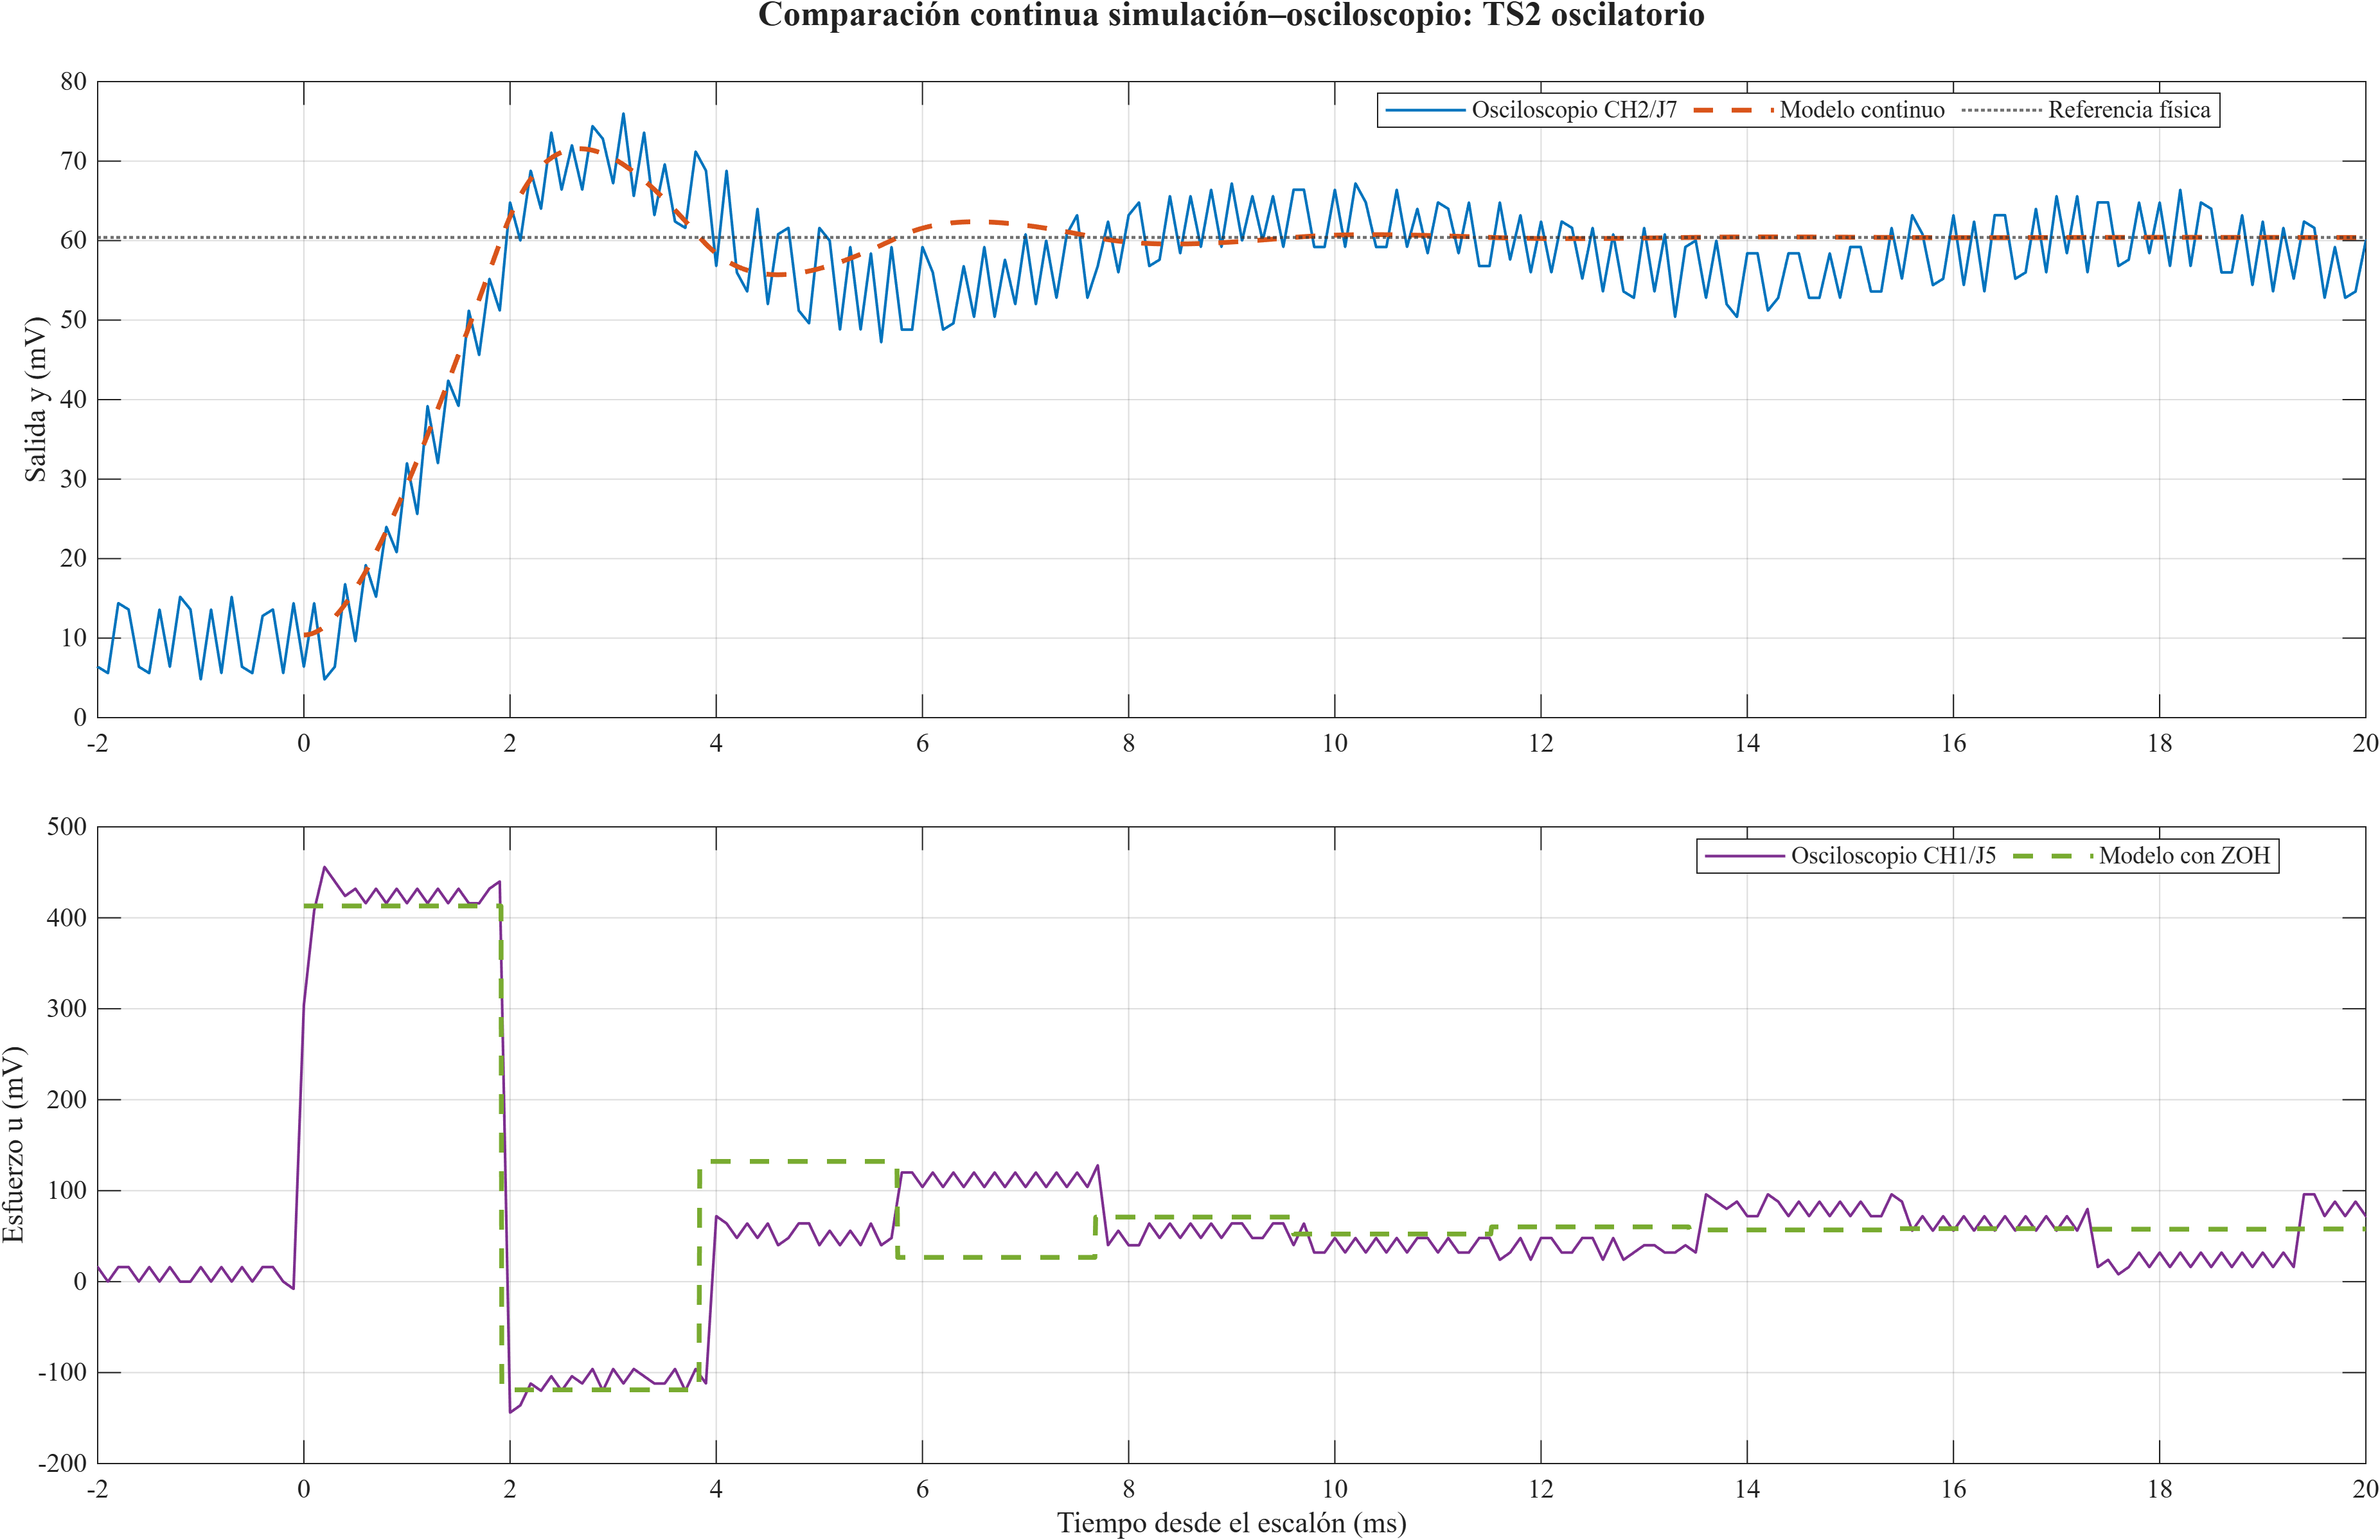
\includegraphics[width=0.78\textwidth]{comparacion_continua_ts2_oscilatorio.png}
\caption{Comparación continua modelo--osciloscopio para TS2 oscilatorio: salida en J7 y esfuerzo de control en J5.}
\vspace{6pt}
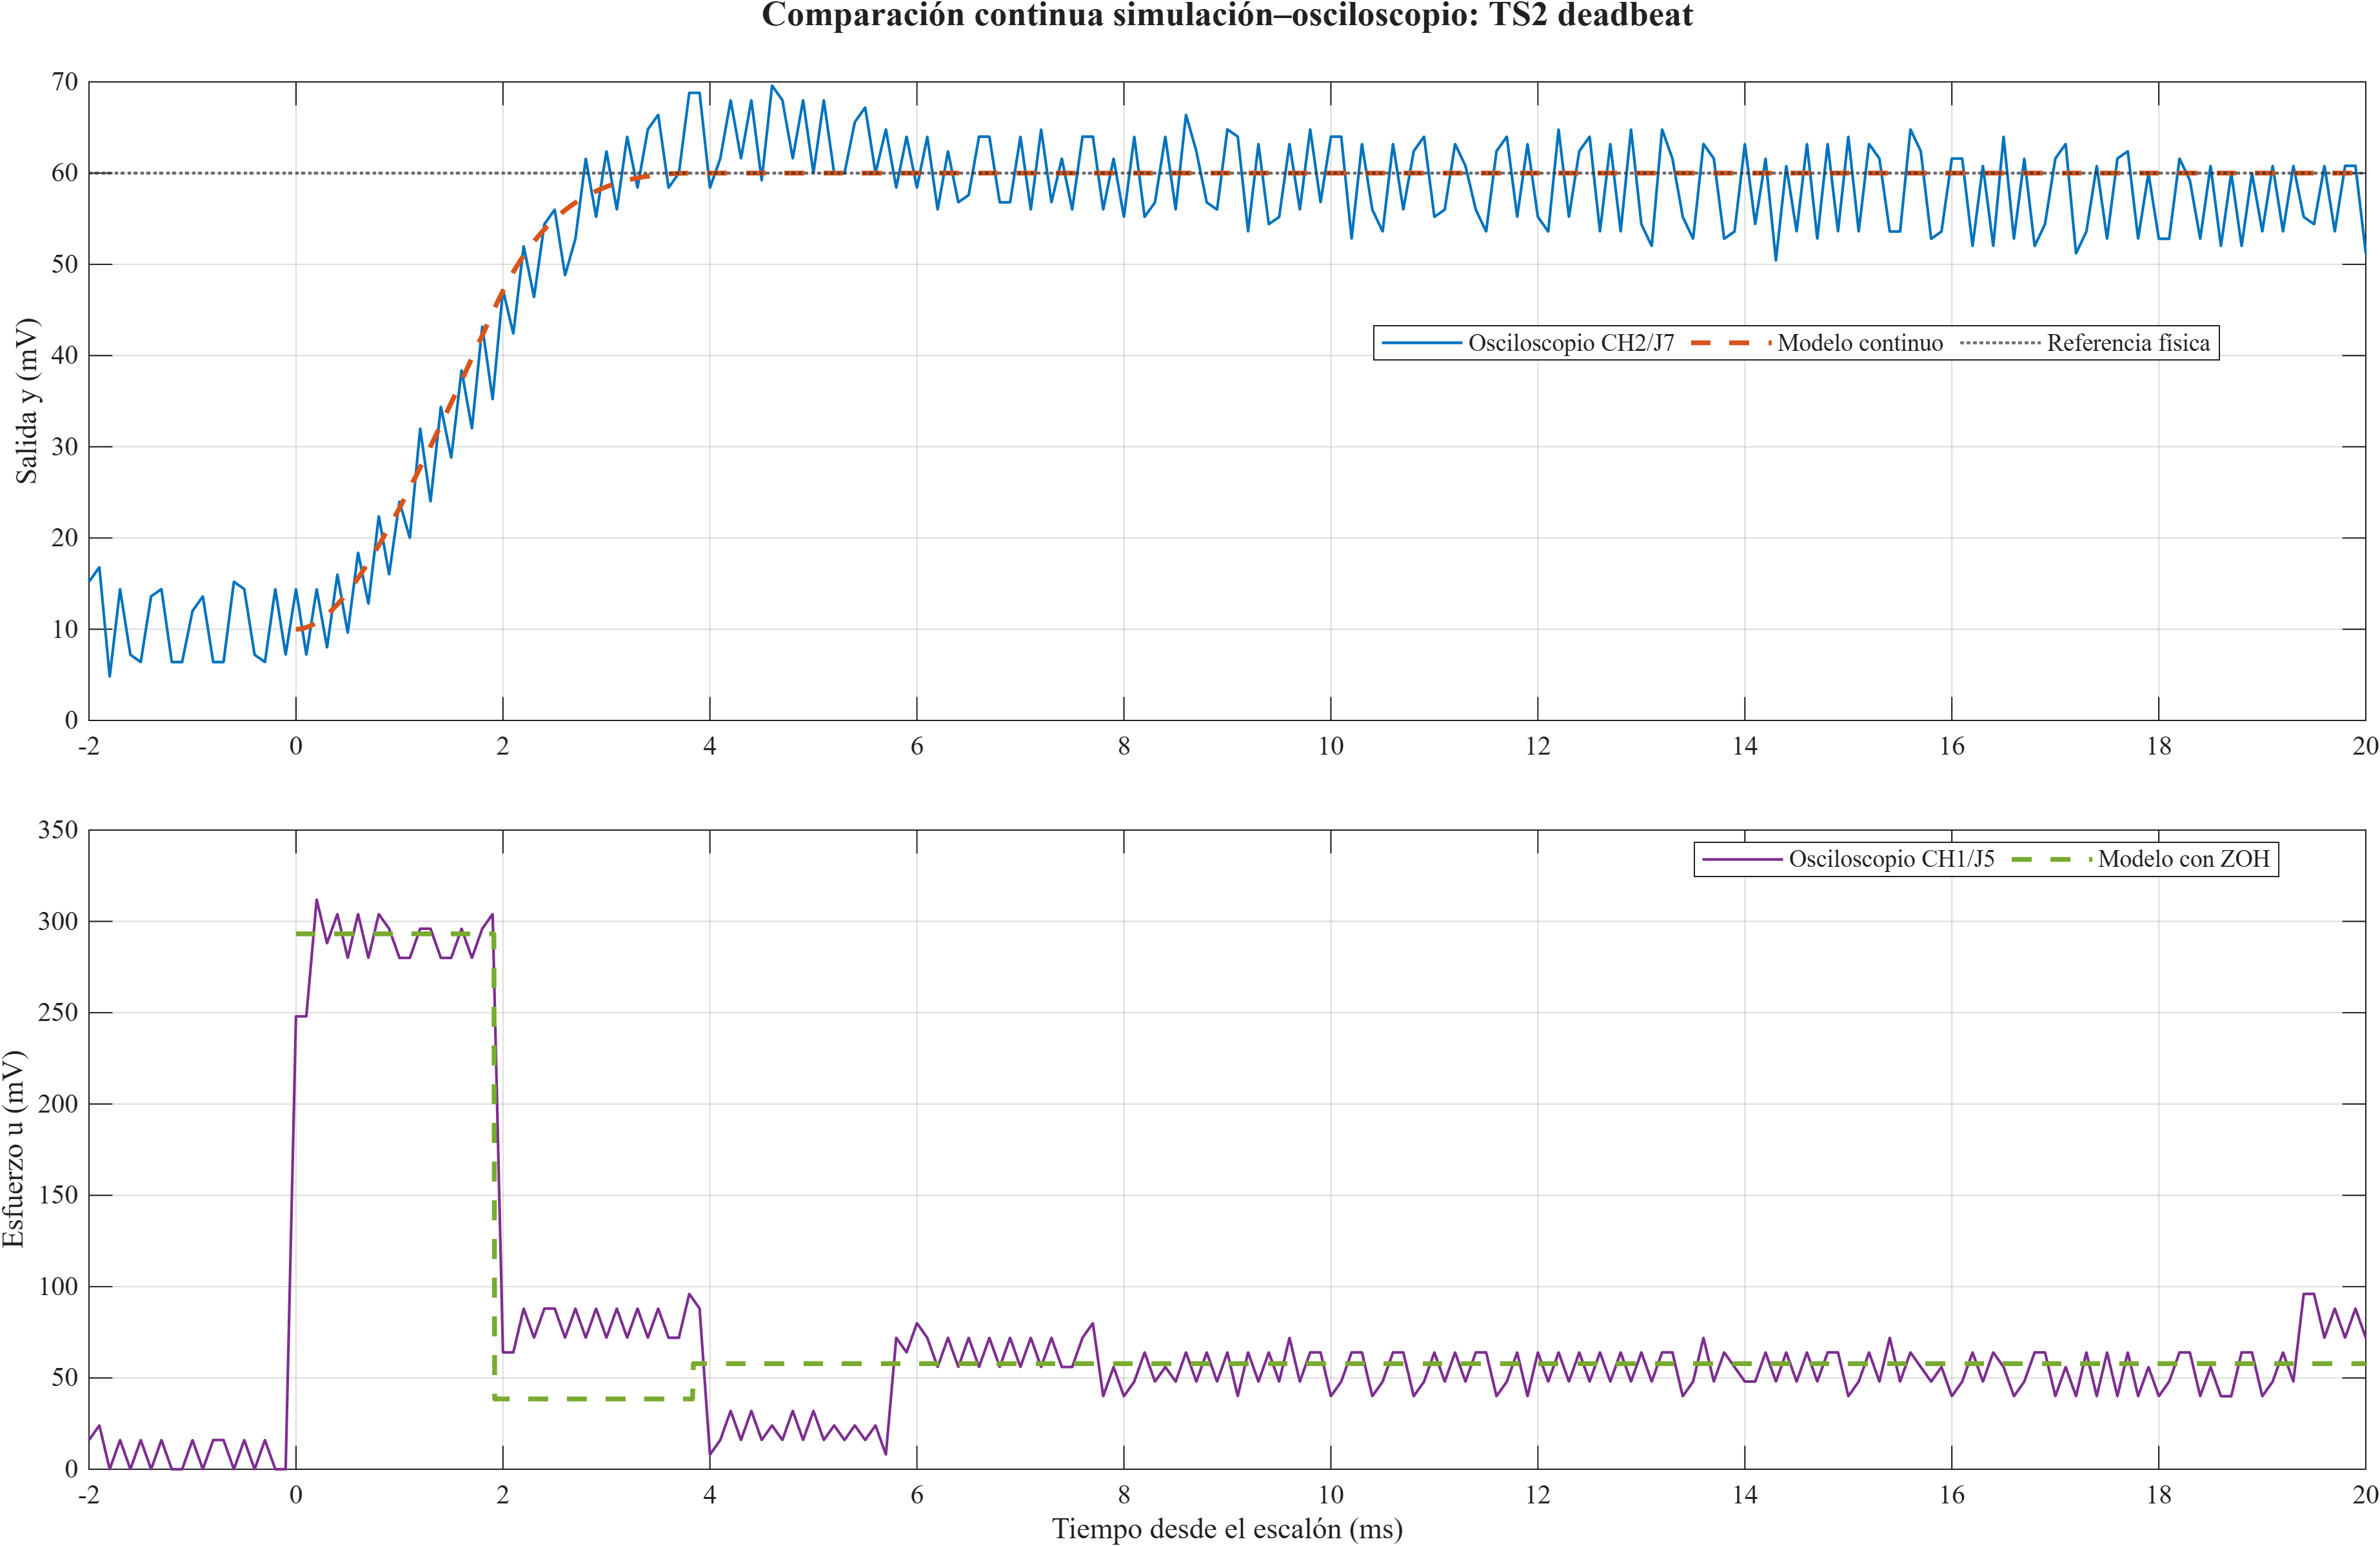
\includegraphics[width=0.78\textwidth]{comparacion_continua_ts2_deadbeat.png}
\caption{Comparación continua modelo--osciloscopio para TS2 deadbeat: salida en J7 y esfuerzo de control en J5.}
\end{figure*}

\clearpage

\subsection{Sensibilidad al ruido de medición}
La transferencia desde el ruido de medición hasta el esfuerzo de control es
\begin{equation}
\frac{U(z)}{N(z)}=-\frac{C(z)}{1+C(z)G_d(z)}.
\end{equation}
Su ganancia máxima, alcanzada cerca de Nyquist, es 3,254 para TS1 deadbeat y 11,184 para TS2 deadbeat. La reducción de \(\Ts\) multiplica por 3,44 la amplificación de ruido del diseño deadbeat. En los controladores oscilatorios, las ganancias máximas son 4,117 y 27,405. Por ello, pequeñas variaciones de la lectura del ADC generan oscilaciones residuales aunque el mando ideal se vuelva constante en tiempo finito.

\subsection{Tiempo de establecimiento físico}
Alcanzar \(r[k]\) en una o dos muestras no determina por sí solo el tiempo de establecimiento de la planta. Mientras el mando siga alternando, la salida continua puede abandonar la banda entre \(k\Ts\), aun si las muestras coinciden con la referencia. En consecuencia, un controlador de una muestra puede presentar un establecimiento físico mayor que otro de dos muestras. Las trazas continuas, el esfuerzo máximo y la sensibilidad al ruido son criterios más adecuados que el número aislado de muestras.

\section{Discusión}
Reducir \(\Ts\) mientras se impone que la referencia se alcance en una muestra exige un tiempo de subida cada vez menor. El efecto es conceptualmente semejante a aumentar en exceso la ganancia de un PID: la respuesta nominal se acelera, pero crecen el esfuerzo y la tendencia a oscilar. En este caso, las oscilaciones son más problemáticas porque ocurren entre muestras, donde el controlador digital no puede observarlas ni actualizar \(u[k]\). El máximo positivo de J5 aumentó de 134 mV en TS1 oscilatorio a 456 mV en TS2 oscilatorio.

La explicación algebraica aparece en el cero introducido por el retenedor. Al pasar de 5,750 a 1,920 ms, dicho cero se desplaza de \(-0,1171\) a \(-0,4204\) y avanza hacia \(z=-1\). Al invertir la planta discretizada, ese cero se convierte en un polo del esfuerzo de control y la componente alternante decae más lentamente en términos del número de muestras. Una actualización más frecuente no elimina este modo; obliga a la planta a reproducir una trayectoria más agresiva.

La formulación deadbeat cancela la cola alternante determinista, pero no el efecto del ruido. La ganancia de la transferencia ruido--control es 11,184 en TS2 deadbeat, frente a 3,254 en TS1 deadbeat. Esta sensibilidad explica el rizado residual de J5 sin contradecir la propiedad deadbeat, que supone modelo exacto y medición sin ruido.

El desplazamiento de continua no se atribuye al método de síntesis. La compensación por pretrigger corrige el nivel medido de la salida, mientras que la inversión de la calibración afín corrige la actuación. Mantener ambas operaciones explícitas evita confundir un ajuste de offset con una normalización de resultados.

No existe un controlador universalmente mejor sin una función de desempeño. Si se prioriza rapidez y el actuador dispone de margen, TS2 deadbeat ofrece la transición más breve; sin embargo, requiere más esfuerzo y presenta 3,44 veces la ganancia de ruido de TS1 deadbeat. Si se penalizan esfuerzo y sensibilidad, TS1 deadbeat es preferible entre los cuatro ensayos: su máximo continuo de J5 fue 120 mV y la ganancia ruido--control fue 3,254, a costa de una respuesta más lenta. La selección definitiva debe fijar límites de establecimiento continuo, esfuerzo máximo y ruido admisible.

\section{Conclusiones}
La síntesis directa produjo cuatro controladores estables y realizables. La respuesta de una muestra alcanza la referencia en los instantes de muestreo, pero conserva en el mando el modo alternante asociado al cero de la planta discretizada. La formulación deadbeat evita esa cola en condiciones ideales. Al reducir \(\Ts\) de 5,750 a 1,920 ms, el cero pasó de \(-0,1171\) a \(-0,4204\), la dinámica exigida se volvió más rápida y el esfuerzo continuo del diseño oscilatorio aumentó de 134 a 456 mV.

Las repeticiones TS1 resolvieron la inconsistencia del archivo original: las cabeceras registraron TS1\_OSCILLATORY y TS1\_DEADBEAT con sus respectivos coeficientes, y ambas trazas fueron capturadas mediante disparo físico. En ese período, el deadbeat redujo el máximo continuo de J5 de 134 a 120 mV. Para TS2, la reducción fue de 456 a 312 mV, es decir, 31,6\,\%.

La enseñanza central es que alcanzar la referencia en \(k\Ts\) no equivale a establecer la planta. Un controlador de una muestra puede seguir oscilando entre muestras y presentar un establecimiento físico mayor que otro de dos muestras. Además, el deadbeat experimental conserva rizado debido a la amplificación del ruido: al disminuir \(\Ts\), su ganancia máxima aumentó de 3,254 a 11,184. Con un criterio que penalice simultáneamente esfuerzo y sensibilidad, TS1 deadbeat ofrece el compromiso más conservador; si la prioridad fuera exclusivamente la rapidez, la decisión podría cambiar.

\section*{Referencias}
\begin{enumerate}[label={[\arabic*]},leftmargin=1.6em,itemsep=0pt,topsep=1pt]
\item K. Ogata, \textit{Sistemas de control en tiempo discreto}, 2.ª ed. Prentice Hall, 1996.
\item G. F. Franklin, J. D. Powell y M. L. Workman, \textit{Digital Control of Dynamic Systems}, 3rd ed. Addison-Wesley, 1998.
\end{enumerate}
\thispagestyle{ultima}
\end{document}
